\documentclass[11pt,a4paper]{scrbook}
\usepackage{geometry}	
\usepackage[utf8]{inputenc}
\usepackage[T1]{fontenc}
\usepackage[pdftex]{graphicx}
\usepackage[ngerman, english]{babel} % the language specified at the end of the list will be used !!
\usepackage{colortbl}	
\usepackage{soul}
% For APA referencing style
\usepackage[natbibapa]{apacite}
\bibliographystyle{apacite}
\usepackage{textcomp}

\renewcommand{\familydefault}{\sfdefault}
\usepackage{xcolor}
\definecolor{uhhred}{cmyk}{0,100,100,0}
\usepackage{float}
\usepackage[ddmmyyyy]{datetime}
\usepackage{comment}
\usepackage[acronym,nomain]{glossaries}

\specialcomment{tobi}{\begingroup\sffamily\color{blue}\commentstyle=\color{codegreen},}{\endgroup}
\specialcomment{shan}{\begingroup\sffamily\color{red}}{\endgroup}

% Generate the glossary
\makeglossaries
 
%%%%%%%%%%%%%%%%%%%%%%%%%%%%%%%%%%%%%%%%%%%%%%%%%

\newacronym{ER}{ER}{Emotion Recognition}
\newacronym{EEG}{EEG}{Electroencephalography}
\newacronym{ADR}{ADR}{Action Design Research}
\newacronym{MTCNN}{MTCNN}{Multi-Task Cascaded Convolutional Neural Network}
\newacronym{AAM}{AAM}{Active Appearance Model}
\newacronym{NN}{NN}{Neural Network}

%%%%%%%%%%%%%%%%%%%%%%%%%%%%%%%%%%%%%%%%%%%%%%%%%%

\begin{document}

\frontmatter  % The \frontmatter declaration makes the pages numbered in lowercase roman
\newgeometry{centering,left=2cm,right=2cm,top=2cm,bottom=2cm}
\begin{titlepage}

\includegraphics[scale=0.3]{UHH-Logo_2010_Farbe_CMYK.pdf}
\vspace*{2.0cm}
\Large
\begin{center}
{\color{uhhred}\textbf{\so{MASTER THESIS}}}
\vspace*{1.0cm}\\
{\textbf{at the University of Hamburg in the Department of Computer Science in the master's programme IT Management and Consulting}}
\vspace*{2.0cm}\\
{\LARGE \textbf{Title:}}
\vspace*{0.4cm}\\
{\LARGE Visual Emotion Recognition In-The-Wild}
%{\LARGE Visual Emotion Recognition In-The-Wild: Prediction of Valence/Arousal and Assessment of Application scenarios}
%{\LARGE Identifying customer intentions in real-time video consultations through emotion recognition: Analysis of viability and value co-creation by implementation of a prototype}
\vspace*{1.5cm}\\
presented by
\vspace*{0.4cm}\\
Tobias Kick
\end{center}
\vspace*{2.0cm}

\noindent
MIN-Faculty \vspace*{0.25cm} \\
Department of Computer Science\vspace*{0.25cm} \\
Program: IT Management and Consulting\vspace*{0.25cm} \\
Research group: Computer Vision\vspace*{0.25cm} \\
Matriculation number: 7213712 \vspace*{0.5cm} \\
%Submission date: 15/12/2020 \vspace*{0.5cm} \\  
Supervisor: Noha Sarhan \vspace*{0.25cm} \\
First assessor: Prof. Dr. Simone Frintrop \vspace*{0.25cm} \\
Second assessor: Prof. Dr. Tilo Böhmann

\end{titlepage}

\restoregeometry

%%%%%%%%%%%%%%%%%%%%%%%%%%%%%%%%%%%%%%%%%%%%%%%%%%%%%%%%%%%%


\chapter{Abstract}
Here is the abstract

%%%%%%%%%%%%%%%%%%%%%%%%%%%%%%%%%%%%%%%%%%%%%%%%%%%%%%%%%%%%

\tableofcontents

\printglossary

%%%%%%%%%%%%%%%%%%%%%%%%%%%%%%%%%%%%%%%%%%%%%%%%%%%%%%%%%%%%
%%%%%%%%%%%%%%%%%%%%%%%%%%%%%%%%%%%%%%%%%%%%%%%%%%%%%%%%%%%%
\mainmatter

%%%%%%%%%%%%%%%%%%%%%%%%%%%%%%%%%%%%%%%%%%%%%%%%%%%%%

\chapter{Introduction}

% What makes this topic so important?
Emotion Recognition through the observation of facial expression is a current trend in Artificial Intelligence. Even though big strides are still to be made in this research area, it already finds its way into concrete business applications. As \citet{Chen:2020:EmotionAI} claim, Emotion Recognition is already being deployed in a variety of different scenarios, such as classrooms and courtrooms. They highlight the adoption of Emotion Recognition in AI-assisted hiring software, especially in the US and South Korea, where new applicants have to interview online with an algorithm. These video interviews are then analyzed with Emotion Recognition in order to figure out a candidate's employability score.
\newline\newline
These applications of technological advances in Emotion Recognition show that this technology has a big optimization and innovation potential. This is why the Hamburg-based software and consulting firm PPI AG regards Emotion Recognition as a technology that can play a very important role for its clients in the banking and insurance industry. The cooperation with PPI AG for this Master's thesis brings in another interesting aspect about the viability of technological advances in the field of Emotion Recognition for a possible application In-The-Wild. An initial analysis of the field (in cooperation with PPI AG) determined that video call consultations between customers as the highest-value application scenario for Emotion Recognition, where it could help assist consultants and customers.
\newline\newline
PPI AG, in its commitment to continuously offer innovative solutions to their clients, is looking for new ways to harness technological advances such as Emotion Recognition in order to apply them in real business scenarios. In that vein, PPI AG aims to better serve their customers, create profitable business solutions and to differentiate themselves from competitors. A basis of this builds the scientific examination of the viability of Emotion Recognition In-The-Wild. Given that the field of Emotion Recognition is still relatively new, there are shortcomings in terms of the research available.
\newline\newline
The current gaps in the research within this field are the following:\newline
\begin{itemize}
    \item As supported by \citet{Salah:2018:VideoBasedER} emotions are inherently cultural and personal, making the task of universally interpreting them very difficult. which makes it very difficult to interpret them in a universal way. Even if emotions were universal, there is still the conflict of representing emotions for Machine Learning systems. On the one hand, these representations should carry higher information, but should on the other hand also be easily interpretable by humans.
    \item Another problem with current research is that most research is done in laboratories, under controlled and predictable conditions (e.g., a perfectly-illuminated face of a person).
    \item There is a significant lack of knowledge about fine-tuning Deep Convolution Neural Networks (DCNN). While \citet{Kossaifi:2017:AFEW-VADatabase} found that DCNNs performed worst under all their examined approaches, \citet{Handrich:2020:SimultaneousPredVA}, on the other hand, are showcasing results in favor of FT-DCNNs.
    \item It is unclear which modules and frameworks work specifically for recognizing emotions with In-The-Wild data.
    \item The lack of focus on business opportunities with Emotion Recognition can also be seen as a research gap, as more research is needed on how to utilize emotions for more commercial purposes.
\end{itemize}

While it is possible to recognize emotions from various input signals, such as facial expressions, speech patterns, and keystrokes, this prototype will be focusing primarily on the recognition of emotions from facial expressions. This simplifies the study, and allows for an easier understanding of the components and modules involved in Emotion Recognition. Furthermore, it will allow for a better comparison of the results achieved. 
\newline\newline
% What is the general topic? 
The main objective of this Master's thesis is to implement a prototype that is able to visually recognize human emotions in-the-wild. The goal of this prototype is to act as a demonstration tool for illustrating the commercial benefits of utilizing an Emotion Recognition software, especially during real-time video calls. 
\newline\newline
% What is my research goal/hypothesis? 
The research will be guided by the following hypotheses: 
\begin{itemize}
    \item Emotions can be recognized reliably from In-The-Wild data used for training and testing. Furthermore, the results could even possibly beat the state-of-the-art outcomes demonstrated in current literature.
    % Question 1: How can the proposed approach be compared to state-of-the-art literature and how well does it perform on in-the-wild data?
    % 1) If: Usage of state-of-the-art 3rd party tools -- Then: Recognize emotions as well as the state-of-the-art literature on in-the-wild data
    \item When examining the implemented modules separately, each module contributes positively towards the performance of the overall architecture.
    % Question 2: How do the implemented modules contribute towards the success of the Machine Learning model?
    % 2) If: Modules are considered separately -- Then: single modules contribute positively towards the performance of the overall architecture.
    \item In a prototype application, Emotion Recognition will perform well with real-time video input from a webcam. It will be able to map recognized emotions to human intentions effectively.

    % Question 3: Can the achieved results be applied for identifying human intentions in a prototype application?
    % 3) If: recognizing emotions from a webcam stream -- Then: human intentions identification
\end{itemize}

% How do I prove the above hypothesis? What do I use as a basis/dataset?
% How would my research supplement the flaws/gap in existing research?
Proving these hypotheses will be further discussed in the \textbf{Methodolgy} chapter, where the researcher will be presenting the proposed approach in concrete and palpable steps -- from the image input to its output. At the core of the approach is the Neural Network, which will be explained in detail in the \textbf{Implementation} chapter. The Neural Network will be trained on the In-The-Wild AFEW-VA dataset containing In-The-Wild video clips, mainly from talk shows and movies.
\newline\newline
In the \textbf{Results and Analysis} chapter, achieved outcomes will be discussed and compared to current state-of-the-art results. This will supplement the gaps in existing literature by providing further insights into the process of fine-tuning DCNNs when handling In-The-Wild data. As an extension of this, in the \textbf{Ablation Study} section, a profound analysis is done for the most important modules, in order to illuminate the contributions for each module, separately. The insights obtained through this analysis will contribute towards expanding the knowledge about the positive impact of single modules/frameworks on the performance of Emotion Recognition with In-The-Wild data.
\newline\newline
In the \textbf{Application} chapter, the achieved results will be implemented in an application prototype that can demonstrate real-time viability of such an approach. This will create scientific evidence that will support the maturity of Emotion Recognition for specific business application scenarios.\newline
Moreover, a user experiment will be conducted that compares the predicted interest based on emotions recognized from facial expressions with the stated level of interest by participants. In this way, conclusions can be drawn about a suspected correlation between Emotion Recognition and human interest. This will supplement research gaps on the utilization of emotion information for the identification of human interest. 
\newline\newline
% What will my contribution to the scientific community be?
This study's overall contribution to the scientific community can be summarized by the following three points:
\begin{itemize}
    \item Performance of Multi-Phase Fine-Tuning vs. Single-Phase Fine-Tuning in the field of Emotion Recognition In-The-Wild
    \item Comparison of different ways of dealing with facial landmarks in the field of Emotion Recognition (AAM vs. ASM vs. Landmarks)
    \item Practical insights gained through an experiment on identifying interest by observing people's facial expressions
\end{itemize}

\chapter{Related Work}

\section{Emotion Representation}
A still widely-discussed research question in emotion recognition is the question about how to best represent emotions, or how to model affect. \citet{Gunes:2011:EmotionRepresentationContinuous} stated that current approaches stem from research in psychology, which distinguishes between three major approaches: \textbf{categorical, dimensional, and appraisal-based.}
% According to research in psychology, three major approaches to affect modelling can be distinguished [1]: categorical, dimensional and appraisal-based approach. The categorical approach claims that there exist a small number of emotions that are basic, hard-wired in our brain and recognised universally (e.g., [2]). This theory on universality and interpretation of affective nonverbal expressions in terms of basic emotion categories has been the most commonly adopted approach in research on automatic measurement of human affect.
% \citep{Gunes:2011:EmotionRepresentationContinuous}
\newline\newline
The \textbf{categorical approach} classifies emotions into a small number of discrete categories, universally-recognised. In this approach, there are six or seven categories, namely, 'happy', 'sad', 'fear', 'anger', 'disgust', 'surprise' and sometimes also 'neutral' \citep{Hupont:2010:FacialEmotionsIn2DAffectiveSpace}. Even though there are many other ways to represent emotions, \citet{Salah:2018:VideoBasedER} argued that this approach is still very relevant today, as it is more natural for humans to interpret emotions in that way. This was supported by \citet{Gunes:2011:EmotionRepresentationContinuous} who posited that the theory on universality, as well as the facility of interpretation has made this approach the most commonly adopted in research on automatic measurement of human affect.
\newline\newline
However, \citet{Gunes:2011:EmotionRepresentationContinuous} argued that this categorical approach is not able to capture the complexity of the affective state exhibited by people in complex and subtle ways (e.g., embarrassment).
% However, a number of researchers have shown that in everyday interactions people exhibit non-basic, subtle and rather complex affective states like thinking, embarrassment or depression. Such subtle and complex affective states can be expressed via dozens of anatomically possible facial and bodily expressions, audio or physiological signals. Therefore, a single label (or any small number of discrete classes) may not reflect the complexity of the affective state conveyed by such rich sources of information
% \citep{Gunes:2011:EmotionRepresentationContinuous}
\newline\newline
%The most widely used dimensional model is a circular configuration called Circumplex of Affect introduced by Russell [3]. This model is based on the hypothesis that each basic emotion represents a bipolar entity being a part of the same emotional continuum. The proposed polars are arousal (relaxed vs. aroused) and valence (pleasant vs. unpleasant)
% \citep{Gunes:2011:EmotionRepresentationContinuous}
\citet{Hupont:2010:FacialEmotionsIn2DAffectiveSpace} proposed a widely-used dimensional approach called 'Continuous Affective Space'. Instead of representing emotions in discrete categories, the Continuous Affective Space approach represents emotions as a point in a two-dimensional plane. This approach allowed for the representation of emotion as a combination of two values: valence and arousal. Valence indicates how positive or negative an emotion was, while arousal indicates how calming or exciting an emotion was. \citet{Hupont:2010:FacialEmotionsIn2DAffectiveSpace} claim that this approach allowed them to capture more information by considering intermediate emotional states.
% Hupont, Cerezo, and Baldassarri(2010): Continous Affective Space, mapping emotions into a 2D space allowing them to consider intermediate emotional states (intermediate emotional state = in-between emotions, gradients of emotions e.g., anxiety to fear, horror to disgust [presumably]). This study allowed for the representation of emotions as a point in a plane, instead of mere items in a categorical list.
% Valence (whether emotion is + or -), arousal (strength of the emotion of expression)
% \citep{Hupont:2010:FacialEmotionsIn2DAffectiveSpace}
\newline\newline
However, \citet{Salah:2018:VideoBasedER} objected that it is possible for a complex emotion to be reduced to a point in a valence-arousal region. She used ’love’ to exemplify that positive or negative values can be attributed to an emotion, depending on the context. While 'love' can usually be identified with a positive valence, a concerned expression of a mother looking at her sick child could be mapped to a negative valence. Therefore, \citet{Salah:2018:VideoBasedER} argued that there was still a need to map such points to a semantic space in order for humans to properly interpret the emotion.
% However, categorical and discrete approaches that go beyond the six (or seven, if we include “contempt”) basic expressions are still very relevant, as their interpretation is more natural for humans. Also, it is difficult to reduce a complex emotion to a point or region in the valence-arousal space. For instance, we can claim that “love” is a positive emotion, and has a positive valence, but this is not always the case. Consider the loving, concerned expression of a mother, looking at her sick child, and this becomes obvious. Subsequently, a given image or video can be annotated in the continuous space, but there is still a need for mapping such points to a semantic space, where it can be properly interpreted 
% \citep{Salah:2018:VideoBasedER}
\newline\newline
There are entirely different approaches arguing that the two dimensional affective space is insufficient for representing the variety of emotions accurately. Two such approaches are the Pleasure, Arousal and Dominance (PAD) approach \citep{Gunes:2011:EmotionRepresentationContinuous} and the Valence, Arousal and Dominance (VAD) approach \citep{Verma:2017:3D-VAD}
% Another well-accepted and commonly used dimensional description is the 3D emotional space of pleasure – displeasure, arousal – nonarousal and dominance – submissiveness [4], at times referred to as the PAD emotion space [6] or as emotional primitives [7]
% \citep{Gunes:2011:EmotionRepresentationContinuous}
% The valence-arousal model is insufficient to represent emotions accurately. Thus, they introduce a 3D model, called Valence-Arousal-Dominance.
% \citep{Verma:2017:3D-VAD}
\newline\newline
\citet{Gunes:2011:EmotionRepresentationContinuous} pointed out that a major challenge for utilizing affective data is the annotation process, as there existed no agreed upon universal annotation scheme. Therefore, it cannot be excluded that the annotations possess a personal biases that lean towards the human annotator's personal context and cultural background. Developing an unbiased annotation scheme poses a difficult challenge in practice, as it would need to be unambiguous and facilitate inter-observer agreement.
% A major challenge in affective data annotation is the fact that there is no coding scheme that is agreed upon and used by all researchers in the field that can accommodate all possible communicative cues and modalities. Development of an easy to use, unambiguous and intuitive annotation scheme that is able to incorporate inter-observer agreement levels will indeed ease the heavy burden of the annotation task. Obtaining high inter-observer agreement is another challenge in affect data annotation, especially when (continuous) dimensional approach is adopted.
% \citep{Gunes:2011:EmotionRepresentationContinuous}
\newline\newline
The \textbf{appraisal-based approach} was still considered by \citet{Gunes:2011:EmotionRepresentationContinuous} as an open research question for automatic measurement of affect. The approach consisted of generating emotions through continuous subjective evaluation of the subject's internal state and the state of the outside world.
% In the appraisal-based approach emotions are generated through continuous, recursive subjective evaluation of both our own internal state and the state of the outside world (relevant concerns/needs) [1], [5], [8], [10]. Despite pioneering efforts of Scherer and colleagues (e.g., [11]), how to use the appraisal-based approach for automatic measurement of affect is an open research question as this approach requires complex, multicomponential and sophisticated measurements of change.
% \citep{Gunes:2011:EmotionRepresentationContinuous}


%%%%%%%%%%%%%%%%%%%%%%%%%%%%%%%%%%%%%%%%%%%%%%%%%%%%%%%%%%%%%%%%%%

\section{Emotion Recognition}

\begin{quote}
    Emotion recognition refers in psychology to the attribution of emotional states based on the observation of visual and auditory nonverbal cues. \citep[~p. 3935]{Baenziger:2014:MeasuringERAbility}
\end{quote}
In Computer Science, however, researchers often directly equate facial expressions with peoples emotions. \citet{Barrett:2019:EmotionalFromFacialMovements} claimed that upon a closer examination of existing psychological research, directly tying facial expressions to emotions is unfounded. This is especially true for the categorical approach of emotion representation, as it favors human interpretability over precision. Therefore, the categorical approach assumes that only six or seven basic emotions exist which can be classified by the observation of visual and auditory nonverbal cues.
\newline\newline
It has to be pointed out, however, that even the methods utilized in this work (i.e., looking exclusively at facial expressions, and utilizing the AFEW-VA dataset with its annotations) assumed an inherent stance that facial expressions correspond to a person’s emotion. This raises the following question: how much of a person's facial expression corresponds to actual emotions?
\newline\newline
\citet{Barrett:2019:EmotionalFromFacialMovements} admitted that scientific evidence confirms that people do sometimes smile when happy, frown when sad, or scowl when angry. This is true for more cases than assigning discrete emotion categories by chance. The authors clarified that people scowl, on average, less than 30 percent of the time when they are angry. Conversely, 70 percent of the time people do not even scowl when they are angry. Hence, scowls are only one of many expressions of anger. Assuming that anger is only detected when a person scowls, the detection rate is around 30 percent, which is really low. It is even lower when considering that not every scowl implies the emotion of anger. This is backed up by \citet{Barrett:2019:EmotionalFromFacialMovements} when they stated that similar facial movements can express multiple instances of different emotion categories.
% The available scientific evidence suggests that people do sometimes smile when happy, frown when sad, scowl when angry, and so on, as proposed by the common view, more than what would be expected by chance.
% People, on average, the data show, scowl less than 30 percent of the time when they’re angry,” says Barrett. “So scowls are not the expression of anger; they’re an expression of anger — one among many. That means that more than 70 percent of the time, people do not scowl when they’re angry. And on top of that, they scowl often when they’re not angry.”
\newline\newline
Furthermore, facial expressions are interpreted differently by various cultures. \citet{Salah:2018:VideoBasedER} stated that in order to establish a ground truth for a facial expression, the cultural background of the subject and the annotator are needed. If there are two annotators from two different cultural backgrounds, the ratings may differ substantially from each other. The authors \citep{Salah:2018:VideoBasedER} cited an experiment with American and Japanese subjects that were asked to annotate facial expression. Even with a closed set of discrete labels the agreement rate was as low as 54.5\% for "fear" and 64.2\% for "anger" annotations. These results proved the existence of a strong annotator bias in every dataset. However, \citet{Salah:2018:VideoBasedER} concluded: whether this is good or bad depends on whether we want the application's algorithm to learn that bias.
% For emotion estimation, we have ample empirical evidence that different cultures interpret facial expressions differently [39]. According to these findings, establishing ground truth for a facial expression database requires the annotation of both the subject and the annotator’s cultural background. If the same database is annotated by, say, Japanese and American subjects, we may get different ratings, unless a very clear, discrete categorization is used. The typical scenario of letting the annotators choose from a closed set of annotation labels may mask the differences in perception, and even when a closed set is used, we see empirical evidence for these differences. In an early study, Matsumoto indeed experimented with American and Japanese subjects, and obtained as low as 54.5% agreement for “fear” annotations and 64.2% agreement for “anger” annotations in Japanese subjects, even with a closed set of discrete labels for annotation [57]. In any case, we may or may not want the algorithm to learn the biases of the annotators, depending on the application. If an algorithm is pre-screening applicants for a job interview selection decision (a highly undesired situation, but may be conceivable for job posts with tens of thousands of applicants), we do not want any biases there
%\citep{Salah:2018:VideoBasedER}
\newline\newline
\citet{Barrett:2019:EmotionalFromFacialMovements} did not only see differences in respect to facial expression interpretation across cultures, but also across different situations and even across people within a single situation. Because of this, companies and institutions that use AI for emotion recognition and base their decisions on these outcomes might inadvertently end up misleading their customers. Therefore, \citet{Barrett:2019:EmotionalFromFacialMovements} were of the opinion that humans need to completely rethink our relationship with emotions, as emotions are varied, complex, and situational. \citet{Barrett:2019:EmotionalFromFacialMovements} compared the needed change in thinking to Charles Darwin's work on the nature of species, as Darwin recognized that each species is a category of highly variable individuals. The same was regarded as true by \citet{Barrett:2019:EmotionalFromFacialMovements} for emotional categories.
% Yet how people communicate anger, disgust, fear, happiness, sadness, and surprise varies substantially across cultures, situations, and even across people within a single situation. 
% \citep{Barrett:2019:EmotionalFromFacialMovements}
% This, in turn, means companies that use AI to evaluate people’s emotions in this way are misleading consumers.
% \citep{Barrett:2019:EmotionalFromFacialMovements}
% Barrett says that perhaps the most important takeaway from the review is that we need to think about emotions in a more complex fashion. The expressions of emotions are varied, complex, and situational. She compares the needed change in thinking to Charles Darwin’s work on the nature of species and how his research overturned a simplistic view of the animal kingdom. “Darwin recognized that the biological category of a species does not have an essence, it’s a category of highly variable individuals,” says Barrett. “Exactly the same thing is true of emotional categories.”
% \citep{Barrett:2019:EmotionalFromFacialMovements}
\newline\newline\newline
\textbf{Technical state-of-the-art}\newline
Despite all the aforementioned considerations about recognizing emotions from facial expressions, researchers are striving to come up with better ways to improve algorithms and their recognition results.
\newline\newline
A notable example is the Facial Action Coding System (FACS) proposed by \citet{Ekman:2002:FACS} which is a way of describing visually discernible facial movements, and is composed of a set of codes, also called Action Units (AUs). These AUs describe the presence and intensity of facial muscle movements. FACS, however, is purely descriptive, it is blind about whether these AUs express any emotions. The descriptive nature of this system can help researchers to better interpret facial expressions.

% In fact, our review of the scientific evidence indicates
% hat very little is known about how and why certain
% acial movements express instances of emotion, par
% cularly at a level of detail sufficient for such conclu
% ions to be used in important, real-world applications.
% \citet{Barrett:2019:EmotionalFromFacialMovements}

% Facial Action Coding System, or FACS (Ekman, Friesen, & Hager, 2002), is a systematic approach to describe what a face looks like when facial muscle movements have occurred. FACS codes describe the presence and intensity of facial movements. FACS is purely descriptive and is therefore agnostic about whether those movements might express emotions or any other mental event.11 Human coders train for many weeks to reliably identify specific movements called action units (AUs). Each AU is hypothesized to correspond to the contraction of a distinct facial muscle or a distinct grouping of muscles that is visible as a specific facial movement.
% \citep{Barrett:2019:EmotionalFromFacialMovements}

Emotion recognition is always based on the observation of subjects in order to attribute them an emotional state. In an optimal scenario, researchers would be able to observe the subjects' thoughts directly. However, the closest researchers got to observing thoughts, is the observation of brain activity through an EEG analysis. \citet{Xing:2019:EEGAudioVisual} did exactly this experiment: they showed video clips to participants, measured the brain activity and fused those measurements with video and audio data. \citet{Xing:2019:EEGAudioVisual} stated that they were able to achieve their best results through this approach.
\newline
While this approach is very promising, the authors pointed out that there was, at the time, no dataset available that obtains EEG signals about emotion activity from participants through video stimulation. Because an EEG is required to produce such a dataset, it would contain no in-the-wild specimens. Needless to say, it would be very difficult to apply such models in real-life situations, as an EEG is not readily available in every household.
\newline\newline
Current researchers base their predictions on more information in an effort to focus on improving the expressiveness of their emotion recognition models. One of the most common approaches that researchers take is finding the best combination of signal fusion (e.g., audio-video and mouse movements). These signal combinations are often supported with extracted features, which help to efficiently characterize the emotional content of the chosen signals. A way of extracting features from video signals could, for example, be the usage of AUs to describe facial muscle movements. 
\newline\newline
Prior to feature extraction in emotion recognition, it is essential to perform face recognition in order to set a bounding box for the person's face. Sometimes the face is recognized by the chosen model architecture at training time, however, when setting a bounding box or detecting landmarks, the facial recognition needs to be performed separately. Nowadays, there are publicly available pre-trained algorithms, like the MTCNN algorithm \citep{Zhang:2016:MTCCN} that perform the task of face recognition, bounding boxing and also landmark detection in one go. As stated by \citet{Zhang:2016:MTCCN}, all these three tasks are somewhat correlated, which is why it makes sense to combine them in one three-layered architecture. The achieved results were better than multiple state-of-the-art architectures from 2016.
% approach: tasks of face detection, bounding boxing and landmark detection are closely related and somehow dependent on each other. Thus they made use of a three layered CNN architecture where they start to detect faces in the first CNN, go over to set the bounding box and then detect the facial landmarks. All this combined in one three-layered architecture, namely MTCNN - Multi-Task Convolutional Neural Network
% This approach delivered significantly better results over multiple state-of-the-art architecture for face detection, alignment and landmark detection from the year 2016.
% \citep{Zhang:2016:MTCCN}
\newline\newline
Combining various signals by fusing them before feeding them into a machine learning model is a common trend in emotion recognition research. The most obvious choice is to combine audio with visual signals, as was done by \citet{Yan:2016:MultiClueFusion} and \citet{Hossain:2019:AudioVisualER}. \citet{Xing:2019:EEGAudioVisual} combined their visual and audio signals with signals from an EEG analysis. All of them argued that their approach achieved significantly better results than their comparison baseline.\newline
Even though it is currently very common that signal fusion happens with video and audio signals, \citet{Akcay:2020:SpeechEmotionRecognition(SER)} pointed out that audio signals could be combined with a wide variety of signals such as visual signals, physiological signals, linguistic features, mouse movements and keystroke dynamics.


%%%%%%%%%%%%%%%%%%%%%%%%%%%%%%%%%%%%%%%%%%%%%%%%%%%%%%%%%%%%%%%%%%%%%%

\section{Identification of Human Intentions}
The ultimate intention of this research is to apply the obtained results from emotion recognition in a real-life application. With that goal in mind, it is important to first lay out the existing state-of-the-art studies on the identification of human intentions through the observation of facial expressions. One of the envisioned purposes of the resulting application prototype will be to use emotion recognition to support consultants during video calls with customers.
\newline\newline
It is of special interest then, for such an application, to be able to identify human intentions. As research is really sparse in that specific area, all the current research related to the identification of human intentions will be presented in the following paragraphs:
\newline\newline
\citet{Dong:2012:UnderstandHumanImplicitIntention} did an experiment where they let participants agree or disagree with a statement. The participants were subjected to an \gls{EEG} analysis in order to measure brain activity. The authors were able to tell by a person’s brain activity whether they agreed or disagreed with a statement even before the person actually vocalized it. Even though the results were very convincing, such an approach would not  be plausible in a real-life setting.
\newline\newline
Another interesting approach was taken by \citet{Esser:2018:LandmarkDetection}. He used facial emotion recognition to visualize the experience of a patient's pain. He made us of an \gls{AAM} for feature extraction in order to better predict the AUs of a person's face. \citeauthor{Esser:2018:LandmarkDetection} was able to measure pain by determining the presence of specific pain-related AUs in a face.
\newline\newline
Identification of customer satisfaction is another practical application of emotion recognition. \citet{Ren:2012:ERforCustomerSatisfaction} ran customers' words and comments through emotion recognition in order to predict emotions and measure the customer satisfaction. While the researchers succeeded in showing the viability of measuring customer satisfaction, it has to be pointed out that they were working under the assumption that accurate emotion recognition results can be directly translated into customer satisfaction.
% Paper from 2012 used customer words and comments to detect customer satisfaction through emotion recognition in this information:
% Using an annotated emotion corpus (Ren-CECps), we
% first present a general evaluation of customer satisfaction
% by comparing the linguistic characteristics of emotional
% expressions of positive and negative attitudes. The associations in four negative emotions are further investigated.
% After that, we build a fine-grained emotion recognition
% system based on machine learning algorithms for measuring customer satisfaction; it can detect and recognize
% multiple emotions using customers’ words or comments.
% The results indicate that blended emotion recognition is
% able to gain rich feedback data from customers, which can
% provide more appropriate follow-up for customer relationship management. \citep{Ren:2012:ERforCustomerSatisfaction}
\newline\newline \citet{Kamaruddin:2016:MeasuringCustomerSatisfaction} took a different approach to identification of customer satisfaction. They predicted emotions from speech signals, and based upon that, they inferred customer satisfaction through a very simple approach: a customer was satisfied if their recognized emotion had a positive value for valence (= a positive emotion), and they were dissatisfied if the value is negative (= a negative emotion). This approach is visualized in figure \ref{fig:SatisfactionFromVA}.

\begin{figure}[htpb]
  \begin{center}
  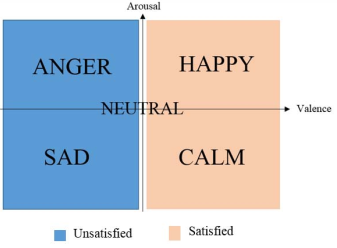
\includegraphics[angle=0, width=0.6\textwidth]{Figures/Satisfaction_from_VA.PNG}
  \caption[Interpretation of emotions]{This graph shows four emotional categories based on valence and arousal, as well as a categorisation in satisfied and unsatisfied. \citet{Kamaruddin:2016:MeasuringCustomerSatisfaction} categorize satisfaction solely based on valence (=how positive or negative an emotion is).}
  \label{fig:SatisfactionFromVA}
  \end{center}
\end{figure}

\citet{Kamaruddin:2016:MeasuringCustomerSatisfaction} realized that using a threshold for defining a 'neutral' region between satisfied and unsatisfied actually performed better in terms of accuracy. However, they admitted that their results were still weak, with 40 \% accuracy for satisfaction determination and 58 \% accuracy for neutral emotion determination. Furthermore, by restricting the outcome to three clasess (stasified, unsatisfied, and neutral) the problem was fairly simplified, but at the same time looses a lot of information.
% In another approach by \citet{Kamaruddin:2016:MeasuringCustomerSatisfaction}, they built upon the hypothesis that the customer is satisfied if he/she is experiencing happiness and neutral emotion whereas if he/she is experiencing sadness or anger, the customer is dissatisfied. They were using Valence and Arousal values and split them up into four emotional values, including one for neutral emotion. They made use of a threshold to define the neutral emotion class. From these classes they directly inferred whether the customer was satisfied or not. Their accuracy stems from the correct prediction of this classes and is with 39 percent accuracy much better than random guessing with 25 percent.
% \begin{quote}
%     We hypothesize that if the valence value is positive (happiness and calm), the customer is satisfied whereas if the valence value is negative (anger and sadness), the customer is not satisfied. Although such approach is simple, it may give us the better understanding of neutral region threshold so that it can be further used for analysis. \citep{Kamaruddin:2016:MeasuringCustomerSatisfaction}
% \end{quote}
\newline\newline
\citet{Poirier:2016:AdsFacialExpression} measured the effectiveness of ads by analyzing facial expressions. \citet{Poirier:2016:AdsFacialExpression} claimed that the emotional journey is the strongest predictor of ad appreciation. The authors predicted the emotional values for valence and arousal, and focused at the curve/profile created by values for valence. Their assumption seemed to be that a certain profile of the valence curve is the main determinant of whether an ad was successful. While this sounds promising, it also raises the question of whether these ad appreciation in commercial ads also converts into actual positive ratings, or even product sales.
% \citet{Poirier:2016:AdsFacialExpression}, the authors measured the effectiveness of ads through facial expressions.
% \begin{quote}
%     emotional journey, which relates to the positive or negative emotional variation  (valence between -1 and 1 where -1: 100\% negative expression, 1: 100\% positive expression and 0: neutral expression), remains the most powerful predictor of ad appreciation 
% \end{quote}
\newline\newline
\citet{Yeasin:2006:MeasurmentOfInterestFromVideo} presented a spatio-temporal approach where they categorized emotions in six classes based on visual data. They mapped those predicted classes to a 3D affect space, and computed the level of interest by calculating L = W x I.  The weight "W" stands for the relative number of images where most motion is concentrated. "I" represents the intensity of an emotion which is calculated by summing up the values for valence, arousal, and stance (3D affect space).
% presents a spatio–temporal approach in recognizing six universal facial expressions from visual data and using them to compute levels of interest. 
% Recognized emotions and used them to calculate a level of interest L, which is calculated as follows: L = W x I. Where I stands for the intensity of an emotion and is calculated through summing up all values from valence, arousal and stance (in a 3D affect space) and mapping these to a range of -5 to +5.
% The weight W is represented by a number in the range of 0 to +1 and measures the relative number of images in a sequence that concentrate most of a motion. The lower the number, the closer the coefficient to 1. \citep{Yeasin:2006:MeasurmentOfInterestFromVideo}



% The FaceReader application \citep{Noldus:2020:Facereader} from Noldus bases their 'Interest' calculation on certain action units instead of recognized emotion values. These action units include:
% \begin{itemize}
%     \item 01 - Inner Brow Raiser
%     \item 02 - Outer Brow Raiser
%     \item 03 - Upper Lid Raiser
%     \item 17 - Chin Raiser
%     \item 20 - Lip Stretcher
%     \item 26 - Jaw Drop
% \end{itemize}
% For the analysis the following time interval is used: Interest - 2 seconds.

\chapter{Methodology}
This chapter covers the proposed emotion recognition approach in detail. First, the components of the pipeline are highlighted briefly, afterwards, each component is described in detail along with justification for the design choices in the following sections. 

\begin{figure}[H]
  \begin{center}
  \makebox[\textwidth][c]{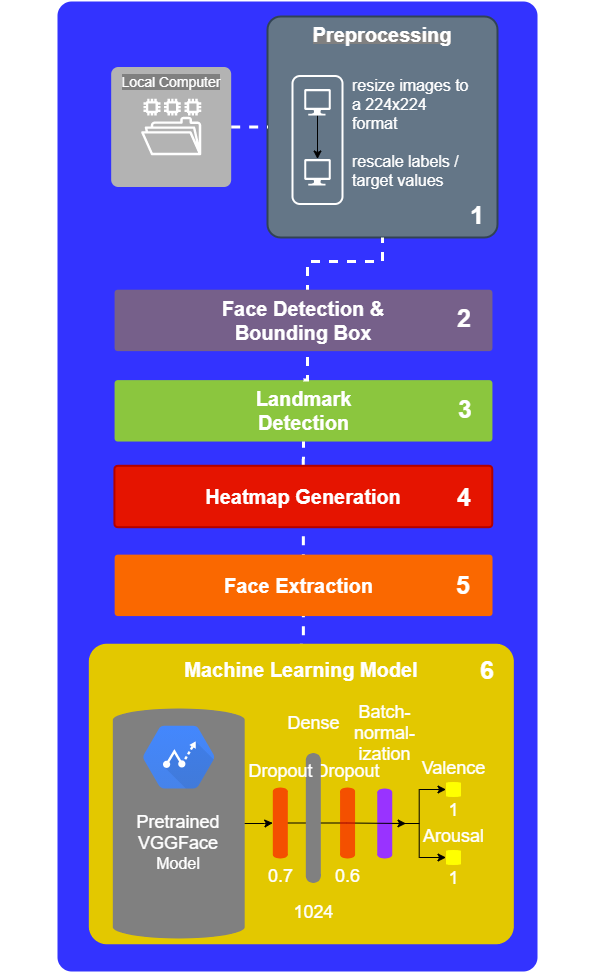
\includegraphics[width=0.55\textwidth]{Figures/DataFlow_Diagram_new.png}}
  \caption{Emotion recognition pipeline in this Master's thesis requires seven essential steps.}
  \label{fig:MachineLearningModelMethods}
  \end{center}
\end{figure}

Figure \ref{fig:MachineLearningModelMethods} illustrates the emotion recognition pipeline in this Master's thesis that consists of six essential steps. First, video frames were resized to a 224x224 format, and data was being standardized by subtracting the training data mean. Second, the face was detected and a bounding box was determined using a pre-trained network optimized for face detection, namely MTCNN \citep{Zhang:2016:MTCCN}. Third, landmarks were detected based on the previously determined bounding box. 
\newline\newline
Fourth, a heatmap was generated using the detected landmarks which was subsequently applied as an overlay to the original image. Fifth, the face was extracted from the image by cropping it along the borders of the bounding box. Sixth, data augmentation was applied in order to significantly increase the diversity of the images in the underlying dataset. Seventh, data was passed into the machine learning model, consisting of a the pre-trained VGGFace neural network that was extended with a custom classifier.

%%%%%%%%%%%%%%%%%%%%%%%
\section{Preprocessing}
The very first step in the pipeline shown in figure \ref{fig:MachineLearningModelMethods} is the preprocessing of both, the input images, as well as the output labels. Input images were resized to the size of 224x224 pixels, as is also required by the pre-trained neural network VGGFace \citep{Cao:2018:VGGFace2}. Output labels, originally in the scale of -10 to +10, were re-scaled to -1 to +1 in order to fit the chosen 'tanh' activation function.
\newline\newline
Samples of the resized input images and their corresponding output labels are shown in figure \ref{fig:MethodologyPreprocess}. Output labels consist of valence (=expression of how positive or negative an emotion is) and arousal (=expression of how strong or weak an emotion is).

\begin{figure}[H]
  \centering
  \subfloat[V: 0.0, A: +0.5]{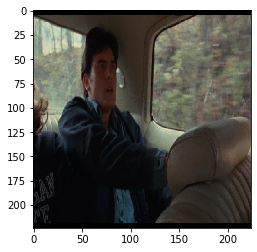
\includegraphics[width=0.33\textwidth]{Figures/preprocessing/001_00000.png}}
  \hfill
  \subfloat[V: +0.2, A: +0.3]{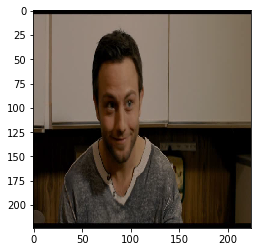
\includegraphics[width=0.33\textwidth]{Figures/preprocessing/002_00000.png}}
  \hfill
  \subfloat[V: -0.5, A: +0.3]{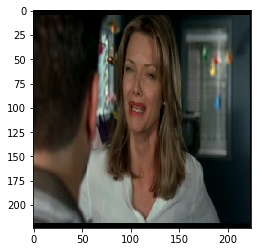
\includegraphics[width=0.33\textwidth]{Figures/preprocessing/576_00000.png}}
  
  \subfloat[V: 0.0, A: +0.5]{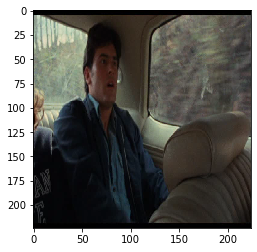
\includegraphics[width=0.33\textwidth]{Figures/preprocessing/001_00011.png}}
  \hfill
  \subfloat[V: +0.2, A: +0.4]{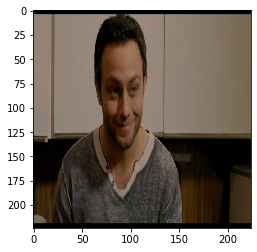
\includegraphics[width=0.33\textwidth]{Figures/preprocessing/002_00011.png}}
  \hfill
  \subfloat[V: -0.6, A: +0.3]{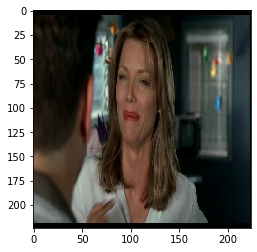
\includegraphics[width=0.33\textwidth]{Figures/preprocessing/576_00011.png}}
  \caption{Preprocessed sample frames from the AFEW-VA dataset \citep{Kossaifi:2017:AFEW-VADatabase} and their corresponding labels representing the valence (V) and arousal (A) as values between -1 and +1.}
  \label{fig:MethodologyPreprocess}
\end{figure}


\section{Face Detection}
The second step in the proposed pipeline involves detecting the faces in each frame of the video. This is valuable in order to determine the face's bounding box which is need in a further stage of the pipeline for the detection of landmarks and the cropping of the image. To achieve this, the Multi-Task Cascaded Convolutional Neural Network (MTCNN) by \citet{Zhang:2016:MTCCN} was used.
\newline\newline
MTCNN is a pre-trained neural network optimized for the tasks of simultaneous face detection, face alignment, bounding boxing and landmark detection \citep{Brownlee:2019:VggFace2HowToFaceRec}. This makes it ideal for the purpose of determining the face's bounding box in the face of the video frames. In figure \ref{fig:MethodologyBoundingBox} successful examples of the application of the MTCNN algorithm are shown by overlaying the bounding box on the image.

\begin{figure}[H]
  \centering
  \subfloat[V: 0.0, A: +0.5]{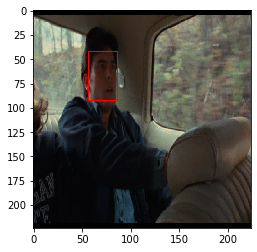
\includegraphics[width=0.33\textwidth]{Figures/boundingbox/001_00000.png}}
  \hfill
  \subfloat[V: +0.2, A: +0.3]{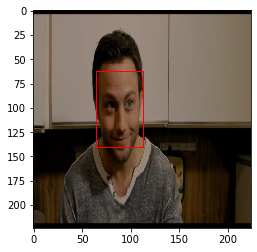
\includegraphics[width=0.33\textwidth]{Figures/boundingbox/002_00000.png}}
  \hfill
  \subfloat[V: -0.5, A: +0.3]{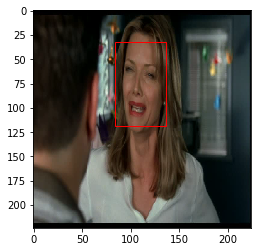
\includegraphics[width=0.33\textwidth]{Figures/boundingbox/576_00000.png}}
  
  \subfloat[V: 0.0, A: +0.5]{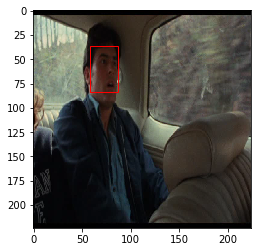
\includegraphics[width=0.33\textwidth]{Figures/boundingbox/001_00011.png}}
  \hfill
  \subfloat[V: +0.2, A: +0.4]{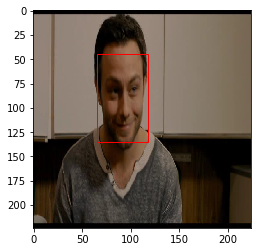
\includegraphics[width=0.33\textwidth]{Figures/boundingbox/002_00011.png}}
  \hfill
  \subfloat[V: -0.6, A: +0.3]{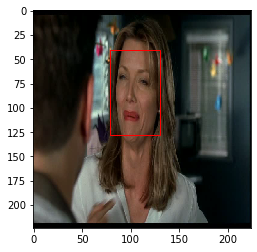
\includegraphics[width=0.33\textwidth]{Figures/boundingbox/576_00011.png}}
  \caption{Visualization of the bounding box detected by the MTCNN face detection module \citep{Zhang:2016:MTCCN} and their corresponding labels representing the valence (V) and arousal (A) as values between -1 and +1.}
  \label{fig:MethodologyBoundingBox}
\end{figure}



\section{Landmark Detection}
The third step in the proposed pipeline involves the detection of facial landmarks in each frame. This is a preliminary step for the generation of the heatmap, as it is based on the coordinates of the landmark points.
\newline\newline
This was done using a 'Face Landmark Detection' algorithm based on the work done by \citet{Kazemi:2014:ShapePredictor}. The algorithm is based on an ensemble of regression trees which successively aligns the constructed shape model to the specific features of the the face at hand.
\newline\newline
The input of the algorithm consists of the frame, as well as coordinates of the face's bounding box. The algorithm's output is made up of 68 facial landmarks of a person's face. Examples of this successful operation are shown in figure \ref{fig:MethodologyLandmarks} by overlaying the landmark dots on the input image.
\citep{Datahacker:2020:DlibFacialLandmarks}

\begin{figure}[H]
  \centering
  \subfloat[V: 0.0, A: +0.5]{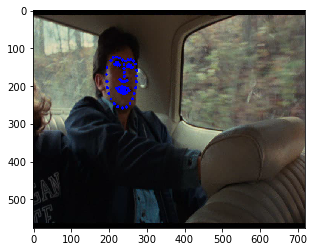
\includegraphics[width=0.33\textwidth]{Figures/landmarks/001_00000.png}}
  \hfill
  \subfloat[V: +0.2, A: +0.3]{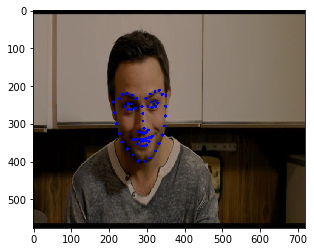
\includegraphics[width=0.33\textwidth]{Figures/landmarks/002_00000.png}}
  \hfill
  \subfloat[V: -0.5, A: +0.3]{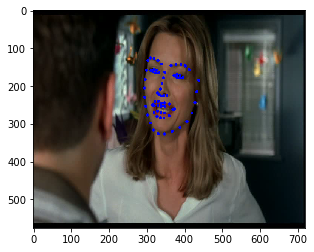
\includegraphics[width=0.33\textwidth]{Figures/landmarks/576_00000.png}}
  
  \subfloat[V: 0.0, A: +0.5]{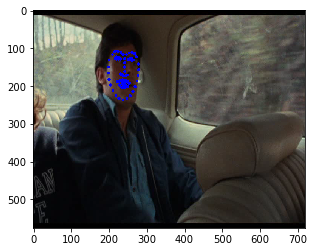
\includegraphics[width=0.33\textwidth]{Figures/landmarks/001_00011.png}}
  \hfill
  \subfloat[V: +0.2, A: +0.4]{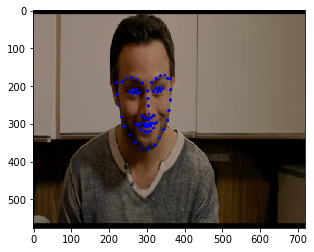
\includegraphics[width=0.33\textwidth]{Figures/landmarks/002_00011.png}}
  \hfill
  \subfloat[V: -0.6, A: +0.3]{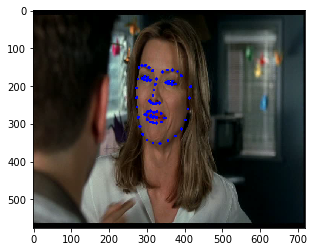
\includegraphics[width=0.33\textwidth]{Figures/landmarks/576_00011.png}}
  \caption{Visualization of the landmarks detected by the pre-trained 'Face Landmark Detection' algorithm \citep{Kazemi:2014:ShapePredictor} and their corresponding labels representing the valence (V) and arousal (A) as values between -1 and +1.}
  \label{fig:MethodologyLandmarks}
\end{figure}


%%%%%%%%%%%%%%%%%%%%%%%%%%%%%%%%%%%%%%%%%%%%%%%%%%%%%
\section{Heatmap Generation}
The fourth step of this work's pipeline involves the conversion of landmarks into a heatmap overlay. This is valuable so that the neural network can learn to differentiate between how important an area is. This was done using an augmentation technique proposed by \citet[~para. 1]{Jung:2020:Imgaug}. Results of this conversion can be seen in the figure \ref{fig:MethodologyHeatmap}.

\begin{figure}[H]
  \centering
  \subfloat[V: 0.0, A: +0.5]{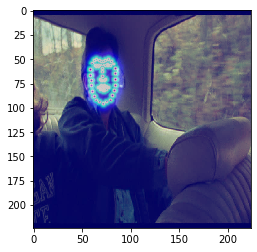
\includegraphics[width=0.33\textwidth]{Figures/heatmap/001_00000.png}}
  \hfill
  \subfloat[V: +0.2, A: +0.3]{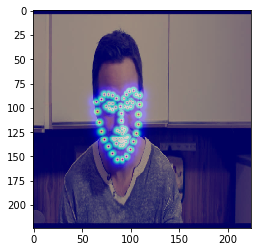
\includegraphics[width=0.33\textwidth]{Figures/heatmap/002_00000.png}}
  \hfill
  \subfloat[V: -0.5, A: +0.3]{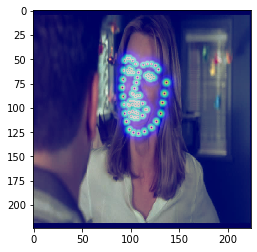
\includegraphics[width=0.33\textwidth]{Figures/heatmap/576_00000.png}}
  
  \subfloat[V: 0.0, A: +0.5]{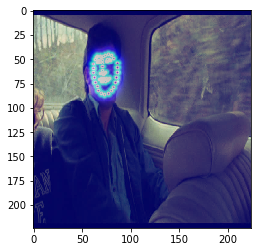
\includegraphics[width=0.33\textwidth]{Figures/heatmap/001_00011.png}}
  \hfill
  \subfloat[V: +0.2, A: +0.4]{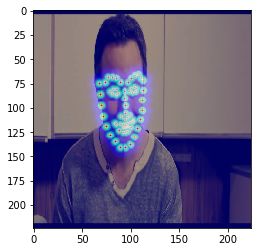
\includegraphics[width=0.33\textwidth]{Figures/heatmap/002_00011.png}}
  \hfill
  \subfloat[V: -0.6, A: +0.3]{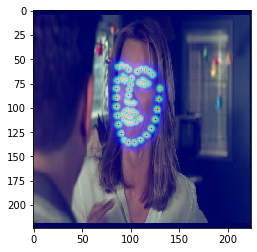
\includegraphics[width=0.33\textwidth]{Figures/heatmap/576_00011.png}}
  \caption{Visualization of the heatmap generated by imgaug algorithm \citep{Jung:2020:Imgaug} and their corresponding labels representing the valence (V) and arousal (A) as values between -1 and +1.}
  \label{fig:MethodologyHeatmap}
\end{figure}


%%%%%%%%%%%%%%%%%%%%%%%%%%%%%%%%%%%%%%%%%%%%%%%%%%%%%
\section{Face Extraction}
The fifth step in the proposed pipeline involves the extraction of the face from the original input image. This is valuable as it removes unimportant information/features of the image's background which could otherwise negatively affect the learning process.
\newline\newline
This step was conducted by simply cropping the face along the border lines of the face's bounding box. The output is again a image with a dimensions of 224x224 pixels that displays the inner area of the bounding box, namely the person's face. Example outputs are illustrated in figure \ref{fig:MethodologyExtraction}.

\begin{figure}[H]
  \centering
  \subfloat[V: 0.0, A: +0.5]{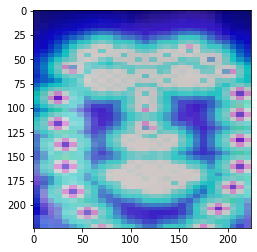
\includegraphics[width=0.33\textwidth]{Figures/extraction/001_00000.png}}
  \hfill
  \subfloat[V: +0.2, A: +0.3]{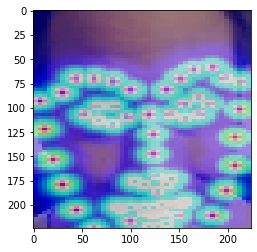
\includegraphics[width=0.33\textwidth]{Figures/extraction/002_00000.png}}
  \hfill
  \subfloat[V: -0.5, A: +0.3]{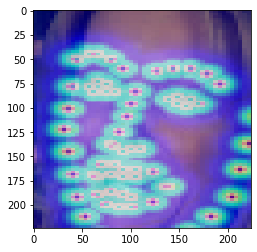
\includegraphics[width=0.33\textwidth]{Figures/extraction/576_00000.png}}
  
  \subfloat[V: 0.0, A: +0.5]{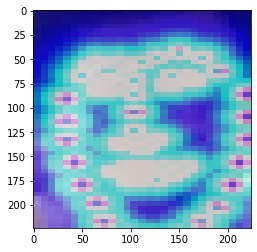
\includegraphics[width=0.33\textwidth]{Figures/extraction/001_00011.png}}
  \hfill
  \subfloat[V: +0.2, A: +0.4]{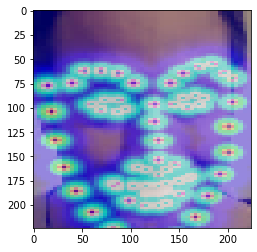
\includegraphics[width=0.33\textwidth]{Figures/extraction/002_00011.png}}
  \hfill
  \subfloat[V: -0.6, A: +0.3]{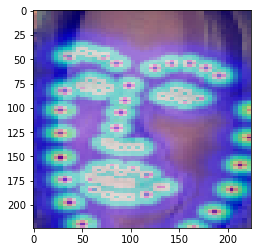
\includegraphics[width=0.33\textwidth]{Figures/extraction/576_00011.png}}
  \caption{Visualization of the extracted face showing the previously applied heatmap, and their corresponding labels representing the valence (V) and arousal (A) as values between -1 and +1.}
  \label{fig:MethodologyExtraction}
\end{figure}


%%%%%%%%%%%%%%%%%%%%%%%%%%%%%%%%%%%%%%%%%%%%%%%%%%%%%
\section{Machine Learning Model for Emotion Recognition}
In the final step of the proposed pipeline, the cropped frames are fed into the machine learning model for training on the emotion recognition challenge. The model's architecture, consisting of the pre-trained VGGFace model \citep{Cao:2018:VGGFace2} and a custom classifier, can be seen in figure \ref{fig:MachineLearningModel}.
\newline\newline
The VGGFace model architecture, is based on the famous ResNet-50 convolutional neural network which the authors \citet{Cao:2018:VGGFace2} pre-trained on a large-scale face dataset, named VGGFace2. The dataset contains about 3.31 million images of 9131 subjects and poses, which provided a wide variety of poses, ages, etc. When the VGGFace2 paper, written by \citet{Cao:2018:VGGFace2}, was published in \citeyear{Cao:2018:VGGFace2}, it exceeded the performance of previous state-of-the-art by a large margin \citep{Cao:2018:VGGFace2}.

\begin{figure}[H]
  \begin{center}
  \makebox[\textwidth][c]{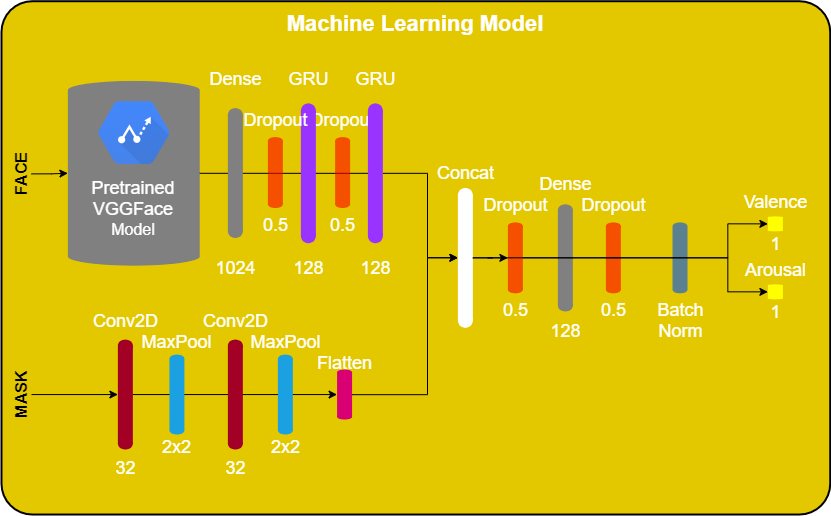
\includegraphics[width=0.6\textwidth]{Figures/MachineLearningModel.png}}
  \caption{The machine learning model consists of the pre-trained VGGFace network where the last layers were replaced by a custom classifier.}
  \label{fig:MachineLearningModel}
  \end{center}
\end{figure}

The utilization of a pre-trained neural network is often referred to as transfer learning. \citet{Pedro:2018:TransferLearning} supports that instead of training the model from scratch, transfer learning allows to start the training process from patterns that have already been learned by solving a different problem.
\newline\newline
In this work, a version of the VGGFace model that was pre-trained on the VGGFace2 dataset \citep{Cao:2018:VGGFace2} for the task of face identification has been used. The pre-trained model was then further fine-tuned on the AFEW-VA dataset \citep{Kossaifi:2017:AFEW-VADatabase}. In this way, learnt patterns about facial features from the face identification task were used to kick-start the learning for emotion recognition from there. 
\newline\newline
A noteworthy architectural change was the removal of the last fully-connected layers at the end of VGGFace. For this work, these layers were replaced with another classifier in order to learn the correlation between facial features and their target labels for the emotion recognition task. The architecture of the newly added classifier is shown in figure \ref{fig:MachineLearningModel}.
\chapter{Implementation}
\section{Experimental setup}
In order to conduct the training process described in the previous chapter, it was necessary to have a computer with a powerful GPU in order to speed up training. For this Master thesis, the experiments/training were conducted on a Nvidia Titan X (Pascal) GPU with 12 GB of memory. 
\newline\newline
For the ease of reproducibility of this work, frameworks and major libraries are hightlighted as follows: For machine learning, Keras 2.2.5 with TensorFlow 1.14.0 as a backend. In addition to that, Keras-VggFace 0.6, MTCNN 0.1.0 and OpenCV 4.1 were used. The entire code was implemented in a Python 3.6 environment.


\section{Dataset}
The selected Acted Facial Expressions in the wild - Valence Arousal (AFEW-VA) dataset introduced by \citet{Kossaifi:2017:AFEW-VADatabase} is based upon the Acted Facial Expressions in the wild database (AFEW) introduced in \citeyear{Dhall:2012:AFEW} by \citet{Dhall:2012:AFEW}. The AFEW dataset is composed of video clips that try to depict a real-world environment. It captures facial expressions, natural head pose movements, occlusions, subjects' races, gender, diverse ages, and multiple subjects in a scene. The authors labeled the video clips with one of six basic expressions: anger, disgust, fear, happiness, sadness, surprise, or neutral. The AFEW-VA dataset \citep{Kossaifi:2017:AFEW-VADatabase} uses the same underlying real-world video data, but it did not annotate its video clips with one of six basic expressions. Instead it used the two dimensional affective space with valence and arousal. 
\newline\newline
Furthermore, as the name of the dataset already suggests, the dataset is compopsed of data that was collected under in-the-wild conditions. In-the-wild refers to real-life conditions in video clips, which make it significantly more challenging to recognize emotions in comparison to a dataset that has been captured in a controlled environment. \citet{Salah:2018:VideoBasedER} explained that these difficulties can be caused by, for example, uncontrolled illumination or uncontrolled video quality due to a different recording medium, like webcams by individuals vs. professional cameras. Such in-the-wild data is usually acquired from talk shows, movies or other natural interactions. 
\newline\newline
Since the research conducted during this Master's thesis is intended to serve as a basis for a further real-life application in video-call scenarios, it was clear that the dataset needed to be as close to in-the-wild conditions as possible. Furthermore, it was decided that it was more important to capture as much of an emotion's information as possible rather than placing value on the interpretation of emotions. As a result, the AFEW-VA dataset got chosen because of its in-the-wild conditions, its 2D Affective Space model for emotion representation and its backing by the scientific community when it comes to providing comparable results.
\newline\newline
The AFEW-VA dataset is made up of 600 video clips, each consisting of multiple frames that make up the video clip. Furthermore, each frame is then annotated in terms of valence and arousal. Both values have an annotation level ranging from -10 to +10 in full integer values. This results in a total of 21 levels.\citep{Kossaifi:2017:AFEW-VADatabase} 


%%%%%%%%%%%%%%%%%%%%%%%%%%%%%%%%%%%%%%%%%%%%
\section{Training \& Regularization}
\subsection{Backbone Network}

\begin{figure}[H]
  \begin{center}
  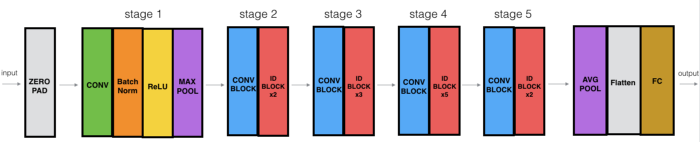
\includegraphics[angle=0, width=1.0\textwidth]{Figures/resnet50.png}
  \caption{ResNet50 \citep{Dwivedi:2019:ResNetInKeras} is a very deep-layered architecture consisting of multiple layers inside each of the five stages.}
  \label{fig:ResNet50Architecture}
  \end{center}
\end{figure}

The chosen ResNet50 model \citep{Dwivedi:2019:ResNetInKeras} consists of 50 layers, combined in 5 stages, and includes over 23 million trainable parameters. It was one of the very first deep-layered neural networks that introduced a solution to the notorious vanishing gradient problem by its 'skip connection' concept.
\newline\newline
'Skip connection' is done by adding a shortcut from the input to the output of a 'CONV' or 'ID' block, allowing the gradient to flow through. This behaviour, as illustrated in figure \ref{fig:ResNet50ConvBlock}, makes sure that the subsequent block performs as least as well as the previous. An overview of the composition of all blocks in ResNet50 is presented in figure \ref{fig:ResNet50Architecture}. 

\begin{figure}[H]
  \begin{center}
  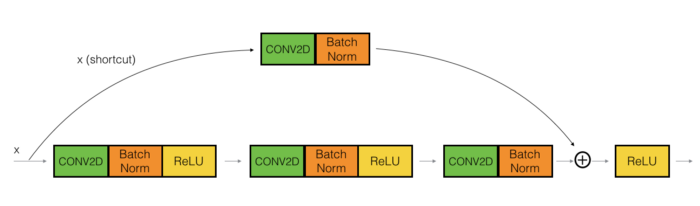
\includegraphics[angle=0, width=0.9\textwidth]{Figures/ResNet50_ConvBlock.png}
  \caption{In a Convolutional block of ResNet50 \citep{Dwivedi:2019:ResNetInKeras}, additionally to adding the result, a convolution is performed on the original input.}
  \label{fig:ResNet50ConvBlock}
  \end{center}
\end{figure}


% ResNet50 is defined by a very deep-layered neural network which traditionally posed a difficult challenge to researchers, as the training process got worse the deeper the neural network due to the notorious vanishing gradient problem. The vanishing gradient leads to a rapid saturation of the model's weights which results in a degradation of the overall model performance. To fight this problem, ResNet introduced a novel concept, named skip connection, where the results of a block are added together with the original input before applying an activation function. \citep{Dwivedi:2019:ResNetInKeras}
% \newline\newline
% This concept is also illustrated in the following figure \ref{fig:ResNet50IdentityBlock} for the identity block:

%\begin{figure}[H]
%  \begin{center}
%  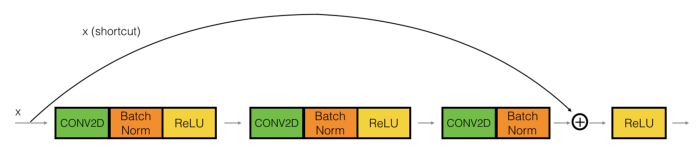
\includegraphics[angle=0, width=0.9\textwidth]{Figures/ResNet50_IdentityBlock.png}
%   \caption{In an Identity block of ResNet50 \citep{Dwivedi:2019:ResNetInKeras}, a shortcut is added by adding the results to the original input.}
%   \label{fig:ResNet50IdentityBlock}
%   \end{center}
% \end{figure}

% However, this operation is only possible when the two inputs for the addition have the same shape. Due to the layout of the ResNet50 architecture, this is inherently the case for the Identity Block. For the Convolution Block a further operation is needed to transform the block's original input into the same shape as the outcome of the Convolutional layers. As can be seen in figure \ref{fig:ResNet50ConvBlock}, this was done by applying a separate Convolutional plus Batch Normalization layer to the original input and choosing its hyperparameters in a way that the output will be in the same shape as the outcome of the Convolutional layers.

% \citet{Dwivedi:2019:ResNetInKeras} argued that this approach is helpful in mitigating the problem of vanishing gradients, as its skip connection concept provided an alternate shortcut path for gradients to flow through. This ensured that the subsequent block will perform at least as well as the previous.




%%%%%%%%%%%%%%%%%%%%%%%%%%%%%%%%%%%%

% \begin{figure}[H]
%   \begin{center}
%   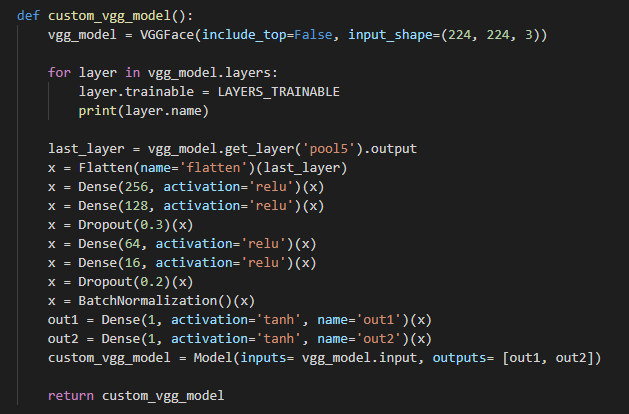
\includegraphics[angle=0, width=1.0\textwidth]{Figures/model_architecture.PNG}
%   \caption{The neural network architecture is constructed by loading the pre-trained VGGFace model and adding a custom classifier.}
%   \label{fig:NNArchitecture}
%   \end{center}
% \end{figure}

% Figure \ref{fig:NNArchitecture} describes the architecture of the neural network with the following elements:

% \begin{itemize}
%     \item Line \#2: the pre-trained VGGFace model is being loaded with 'resnet50' as its neural network architecture. With the parameter 'include\_top' set to False allows to exclude the classifier of the pre-trained network on face detection.
%     \item Line \#5 to line \#10: The VGGFace model is either set to trainable or non-trainable. For the first three epochs of fune-tuning, the model gets set to non-trainable. Afterwards it is set to trainable, and allows the model to update its weights.
%     \item Line \#12: The output of the VGGFace model is being accessed and in line \#13 reduced in dimensionality in order to fit the input requirements for the following layer.
%     \item Line \#15 to line \#18 contains the classifier consisting of a Dense layer (1024 units), together with two Dropout and a Batch Normalization layer in order to improve generalization capabilities.
%     \item Line \#20 and \#21: The output for each evaluation metric is defined individually. This makes it possible to neatly visualize the outcomes separately. The 'tanh' activation function resized the output to a floating-point number in the range of -1 to +1.
% \end{itemize}

% The choice of using only a single Dense layer in the classifier was based on a comparison of fine-tuning strategies by \citep{Pittaras:2017:FineTuningStrategiesComparison}. Through this comparison of fine-tuning strategies on pre-trained neural networks, they could show that
% \begin{quote}
%     increasing the depth of a pre-trained network with one more fully-connected layer and fine-tuning the rest of the layers on the target dataset can improve the network’s concept detection accuracy compared to other fine-tuning approaches. \citep[~p. 103]{Pittaras:2017:FineTuningStrategiesComparison}
% \end{quote}

% Moreover, \citet{Pittaras:2017:FineTuningStrategiesComparison} could obtained their best results with a fine-tuning approach that replaced the pre-trained classifier of a network with a single Dense layer containing a high number of neurons.

%%%%%%%%%%%%%%%%%%%%%%%%%%%%%%%%%%%%%%%%%%%%%%%%%%%%%%%%%

\subsection{Training}
\subsubsection{Pre-trained network}
A pre-trained network is a saved neural network that was previously learned spatial hierarchy of features on a large and general dataset. As recommended by \citet{Chollet:2017:DeepLearningPython} using a pre-trained neural network is a highly effective approach when dealing with a small image dataset. With around 30.000 frames (= 600 video clips), the AFEW-VA dataset \citep{Kossaifi:2017:AFEW-VADatabase} can be considers as such. This is why the VGGFace network, based on ResNet50 and pre-trained on the large-scale face recognition dataset VGGFace2 \citep{Cao:2018:VGGFace2}, was chosen as a basis for this work.

\subsubsection{Fine-tuning}
In order to be able to fine-tune a pre-trained network, it first had to be adapted to the current challenge. Therefore, in this work the classifier got replaced with a single Dense layer. This decision was based on a comparison of fine-tuning strategies conducted by \citet{Pittaras:2017:FineTuningStrategiesComparison} who found out that they achieved the best results fine-tuning results when only adding a single Dense layer with a high number of neurons.
\newline\newline
In the first fine-tuning step, only the classifier was trained on the dataset for a few epochs. According to \citet{Chollet:2017:DeepLearningPython}, this prevents the error being propagated through the network from getting to big, which would have happened when training the whole network from the start. 
\newline\newline
In the second fine-tuning step, the pre-trained neural network was trained in accordance with the selected Multi-Phase Fine-Tuning (FT) \citep{Sarhan:2020:MultiPhaseFineTuning} strategy. In contrast to Single-Phase FT where network is trained by unfreezing a set amount of layers at once, in Multi-Phase FT the network is trained by successively unfreezing layers in phases. This is illustrated in figure \ref{fig:MultiPhaseFT}. According to \citet{Sarhan:2020:MultiPhaseFineTuning} this approach not only reached better accuracy, but also converged in a fewer epochs. 

\begin{figure}[H]
  \begin{center}
  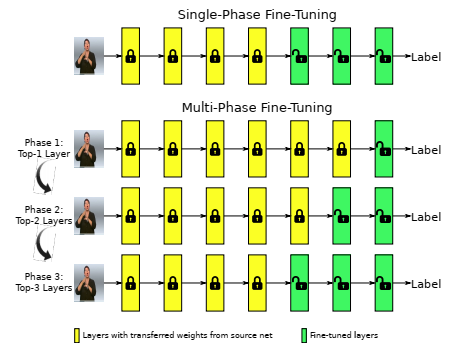
\includegraphics[angle=0, width=0.8\textwidth]{Figures/MultiPhaseFT.PNG}
  \caption{Multi-Phase Fine-Tuning (FT) leads to better accuracy in fewer training epochs in comparison to Single-Phase FT.}
  \label{fig:MultiPhaseFT}
  \end{center}
\end{figure}

%%%%%%%%%%%%%%%%%%%%%%%%%%%%%%%%%%%%%%%%%%%%%%%%%%%%%%%
\subsection{Regularization}
A central role in developing a successful solution with machine learning is making sure that an algorithm will perform well not only on the training data, but also on previously unseen data. In many machine learning challenges it is common, that a well performing algorithm on the training data performs bad on previously-unseen data. This happens when the model is trying to memorize the training dataset, instead of learning its underlying patterns. This behaviour is called 'overfitting'. Strategies explicitly designed for decreasing overfitting, even at the expense of increasing the training error, are known as regularization. \citep{Goodfellow:2016:DeepLearning}
\newline\newline
In order to prevent overfitting and generalize a model better, \citet{Chollet:2017:DeepLearningPython} highlighted that the best solution is to get more training data, because more data means the model needs to learn to represent all data points, thus the lower the chance that it would overfit. However, when it is not possible to expose the model to more data, \citet{Chollet:2017:DeepLearningPython} recommended utilizing regularization techniques, which will force the model to focus on the most prominent patterns. These techniques constrain a model in a way that it can only store a certain amount or a certain type of information. According to \citet{Chollet:2017:DeepLearningPython}, the easiest way to prevent overfitting is to reduce the network's size, or in other words, to remove features. As a result, the number of trainable parameters in the model is reduced and thus, the model's capacity shrinks.

\subsubsection{Feature removal}
For the here proposed machine learning model it was not possible to increase the amount of training data, as this would make an objective comparison with benchmark paper impossible. Thus, further regularization techniques were applied. The first choice was also to reduce the network's size. The pre-trained VGGFace network already provides a big stack of layers that cannot be removed without losing valuable information. Therefore, the custom layers were reduced to a single Dense layer, which was proposed in a similar way by \citet{Pittaras:2017:FineTuningStrategiesComparison}, and Dropout was chosen to make the network purposefully forget some information.

\subsubsection{Dropout}
According to \citet{Chollet:2017:DeepLearningPython}, Dropout is one of the most effective and commonly used regularization techniques. When applied, noise is introduced during training by randomly setting a certain percentage of the layer's output values to zero. The Dropout applied in the proposed architecture was determined through extensive experimentation and was applied before and after the single Dense layer with a rate of 0.7 and 0.6 respectively. The following figure shows an example with a dropout rate of 0.5.

\begin{figure}[H]
  \begin{center}
  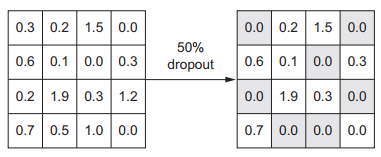
\includegraphics[angle=0, width=0.7\textwidth]{Figures/dropout.PNG}
  \caption{The applied dropout sets a defined percentage share of the parameters of an activation matrix to zero.\citep{Chollet:2017:DeepLearningPython}}.
  \label{fig:Dropout}
  \end{center}
\end{figure}

\subsubsection{Data Augmentation}
Data Augmentation is another technique that is used to increase noise during training by randomly transforming existing training samples into slightly different looking images. As \citet{Chollet:2017:DeepLearningPython} argued that Data Augmentation exposes the model to more aspects of the data, as it will never see the exact same picture twice. As a result, the model will generalize better.
The Data Augmentation applied in the here proposed solution augmented the images randomly with the following parameters:

\begin{itemize}
    \item rotation range from 0 to 30 degrees
    \item width shift range from 0 to 25 percent of the total width
    \item height shift range from 0 to 25 percent of the total height
    \item horizontal flip
    \item brightness shift range from 50 to 150 percent
    \item zoom range from 0 to 30 percent
\end{itemize}


\subsubsection{Hyper-parameter optimization}
Optimization of important hyper-parameters also greatly reduces the effects of overfitting. Two of the most impactful parameters are the learning rate and the batch size.
\newline\newline
An analysis conducted by \citet{Yuanzhi:2019:RegularizationInitialLargeLearningRate} on Initial Learning Rates confirmed that an initially large learning rate can have a regularization effect on the training process. Even though a small initial learning rate might allow for better performance initially, it will not be able to generalize as well as initially large learning rates. The training performed in this Master's thesis made use of an initial learning rate of 0.0001 for the first 3 epochs. Afterwards it was lowered to 0.00001.
\newline\newline
Along with the effects of the initial learning rate on improving generalization and reducing the effects of overfitting, \citet{Keskar:2016:LargeBatchTrainingGeneralization} posited that choosing small-batch methods consistently generalizes better than large batch methods. For the here proposed approach, utilized during 5-fold-cross-validation, made use of a batch size of 16.


%%%%%%%%%%%%%%%%%%%%%%%%%%%%%%%%%%%%%%%%%%%%%%%%%%%%%%%%%

\section{Evaluation \& Metrics}
\subsection{Evaluation}
Both benchmark papers, the AFEW-VA paper proposed by \citet{Kossaifi:2017:AFEW-VADatabase} and the simultaneous VA prediction paper proposed by \citet{Handrich:2020:SimultaneousPredVA}, compare their results through an evaluation on the AFEW-VA dataset that was split into five disjoint and subject-independent folds. Subsequently, they performed a 5-fold-cross-validation for the prediction of valence and arousal values. 
\newline\newline
As illustrated in figure \ref{fig:TrainTestSplit}, in this work the folds were then assigned to three subsets as follows: three folds were combined in the training subset, while validation and testing subsets contained exactly one fold. This setup, without performing 5-fold-cross-validation, was used to conduct various experiments in order to determine optimal hyper-parameter settings.

%\citet{Roehrich:2020:TrainValidateTest} argued that when comparing different models it is not enough to only use a training and a testing subset, as it might still be possible that one model performs better than the other due to randomness during the training process. 


\begin{figure}[H]
  \begin{center}
  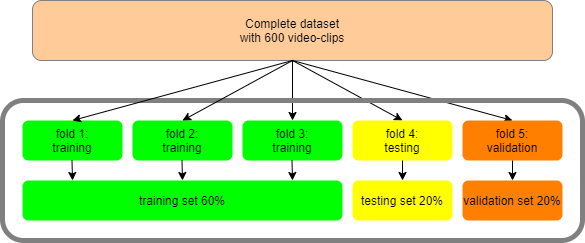
\includegraphics[angle=0, width=0.7\textwidth]{Figures/TrainTestSplit.png}
  \caption{After splitting the dataset into five folds, the folds are assigned to their respective subset.}
  \label{fig:TrainTestSplit}
  \end{center}
\end{figure}

As soon as optimal hyper-parameter settings were found during the training of the model, a 5-fold-cross-validation was conducted in order to make results comparable with the benchmark. For this 5-fold-cross-validation, previously determined optimal hyper-parameter settings were utilized for training the model five times. As illustrated in figure \ref{fig:CrossValidationSplit}, each time the model is trained during cross-validation, a different combination of folds was selected as training, validation and testing subset.\newline

\begin{figure}[H]
  \begin{center}
  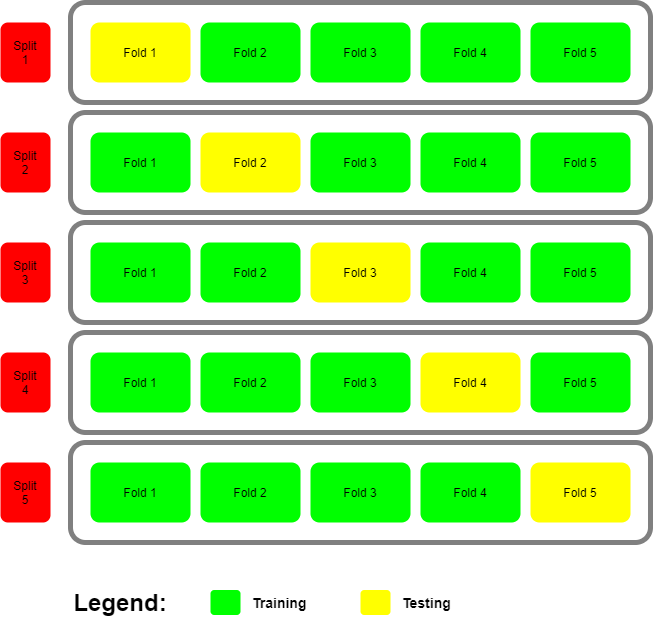
\includegraphics[angle=0, width=0.7\textwidth]{Figures/CrossValSplit.png}
  \caption{The dataset is split into five equal and subject-independent folds. Cross-Validation is performed by alternating the folds for training, validation and testing.}
  \label{fig:CrossValidationSplit}
  \end{center}
\end{figure}

\subsection{Metrics}
Considering the nature of the problem at hand, predicting the values for valence and arousal is better solved through regression, hence a metric such as accuracy, albeit common, will not provide useful information to reflect the performance of the system. Therefore, we stick to the measures used by \citet{Kossaifi:2017:AFEW-VADatabase}, namely root-mean-square error (RMSE) and Pearson product-moment correlation coefficient (CORR). 
\newline\newline
RMSE (eq. \ref{eq:RMSE}) is useful in giving the observer a notion of how close the predicted values are to the actual values, while CORR (eq. \ref{eq:CORR}) tells how strong the relationship between the prediction and the actual label is. \citep{2020:RMSE} \citep{2020:PearsonCorrelation}
  
\begin{equation} \label{eq:RMSE}
RMSE = \sqrt{(\frac{1}{n})\sum_{i=1}^{n}(y_{i} - x_{i})^{2}}
\end{equation}
\newline\newline
\begin{equation} \label{eq:CORR}
CORR = \frac{{}\sum_{i=1}^{n} (x_i - \overline{x})(y_i - \overline{y})}
{\sqrt{\sum_{i=1}^{n} (x_i - \overline{x})^2(y_i - \overline{y})^2}}
\end{equation}

where
\begin{conditions*}
 x_i  &  the actual ground truth value\\
 y_i  &  the predicted output value \\
 \overline{x}  &  the mean of all ground truth values \\
 \overline{y}  &  the mean of all predicted output values
\end{conditions*}

The RMSE is additionally used as the loss function to be for optimization during training.


\subsection{Observation}
% Early Stopping & Model Checkpoint?
The aforementioned metrics applied to the validation data were continuously observed by an early stopping callback, as well as a model checkpoint callback. These made sure that the last best model, in terms of validation loss, was automatically backed up and that training was stopped as soon as the model successively failed to improve. The callbacks for this work are clearly defined in figure \ref{fig:EarlyStopping} and \ref{fig:ModelCheckpoint}.

\begin{figure}[H]
  \begin{center}
  
\includegraphics[angle=0, width=0.8\textwidth]{Figures/EarlyStopping.PNG}
  \caption{The early stopping callback stops the training process as soon as there has not been any learning progress after a set period of epochs.}
  \label{fig:EarlyStopping}
  \end{center}
\end{figure}

\begin{figure}[H]
  \begin{center}
  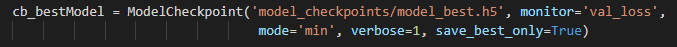
\includegraphics[angle=0, width=0.8\textwidth]{Figures/ModelCheckpoint.PNG}
  \caption{The Model Checkpoint Callback tracks the best performing epoch according to a defined metric and automatically saves the weights of the best model.}
  \label{fig:ModelCheckpoint}
  \end{center}
\end{figure}

In summary, the model checkpoint automatically saves the latest best model in terms of validation loss, while the early stopping callback automatically interrupted the training process after 20 consecutive epochs without showing any improvement.
\chapter{Results and Analysis}
% (more tables and graphs; comparison; what other people achieved)
The following results and studies were based upon the AFEW-VA dataset. Results were compared with the metrics Root-Mean-Squared-Error (RMSE) and Pearson Correlation (CORR). The optimization goal was to reduce the RMSE error while improving the CORR as much as possible.

\section{Benchmark AFEW-VA Dataset}
In the original paper from 2017 where the AFEW-VA database \citep{Kossaifi:2017:AFEW-VADatabase} was introduced, \citet{Kossaifi:2017:AFEW-VADatabase} already provided a benchmark by comparing different methods such as SVR or DCNN, with the following metrics: RMSE (Root Mean Squared Error), CORR (Correlation), and ICC (Interclass Correlation). In the following table, the best performing Deep Neural Network approach is compared with the overall best performing algorithm, called Multiple Kernel Learning (MKL):

\begin{table}[H]
\begin{center}
\begin{tabular}{@{}rcccc@{}}
\toprule
\multicolumn{1}{c}{} &  & RMSE & CORR & ICC \\ \midrule
\begin{tabular}[c]{@{}r@{}} \\FT-DCNN\\ (RGB images)\end{tabular} & Valence & 0.37 & 0.26 & - \\
\begin{tabular}[c]{@{}r@{}} \end{tabular} & \multicolumn{1}{l}{Arousal} & 0.39 & 0.31 & - \\
\begin{tabular}[c]{@{}r@{}} \\ MKL\\ (Shape + DCT)\end{tabular} & \multicolumn{1}{l}{Valence} & 0.264 & 0.40 & 0.27 \\
\begin{tabular}[c]{@{}r@{}} \end{tabular} & Arousal & 0.223 & 0.45 & 0.34 \\ \bottomrule
\end{tabular}
\caption{Benchmark result from AFEW-VA paper}
\label{tab:BenchmarkAFEWVA}
\end{center}
\end{table}

The best performing method in the aforementioned study was the MKL algorithm.The FT-DCNN approach is very similar to the one used in this thesis, and is  a fine-tuned Deep Convolutional Neural Network by training it on randomly sampled frames from video sequences. Fine-tuning is being done with AlexNet, a pretrained model on the ImageNet dataset.
\newline\newline
\citet{Theagarajan:2018:DeepDriver} used the AFEW-VA database to evaluate their approach in their 'DeepDriver' paper. It consisted of taking multiple frames as a sequence and feeding them into either a CNN-only architecture, as well as an CNN + LSTM architecture. Both methods heavily outperformed all benchmark results on the RMSE and CORR metric. The best result, using the CNN + LSTM, achieved the following results:

\begin{table}[H]
\begin{center}
\begin{tabular}{@{}rccc@{}}
\toprule
\multicolumn{1}{c}{} &  & RMSE & CORR \\ \midrule
CNN + LSTM & Valence & 0.09 & 0.64 \\
 & \multicolumn{1}{l}{Arousal} & 0.09 & 0.63 \\ \bottomrule
\end{tabular}
\caption{Benchmark result from DeepDriver paper}
\label{tab:BenchmarkDeepDriver}
\end{center}
\end{table}

These results were obtained using a 3-fold cross validation approach for training and evaluation. However, the author utilized two different datasets, the AFEW-VA and MotorTrend's dataset. Therefore, the training was conducted on two separate datasets, which made the approach objectively incomparable to the approach proposed in this Master's thesis. 
\newline\newline
\citet{Handrich:2020:SimultaneousPredVA} made use of cross-database validation for the recognition of valence and arousal in videos/images. They used the AFEW-VA database \citep{Kossaifi:2017:AFEW-VADatabase} as a validation dataset and achieved much better results for the CORR and ICC metrics. Needless to say, their approach is an improvement form the 2017 benchmark paper. Their proposed CNN architecture is also based upon RGB images as an input. The study achieved the following results:

\begin{table}[H]
\begin{center}
\begin{tabular}{@{}rlcc@{}}
\toprule
\multicolumn{1}{c}{} & \multicolumn{1}{c}{} & RMSE & CORR \\ \midrule
\begin{tabular}[c]{@{}r@{}}AFEW-VA\\ DB only\end{tabular} & \multicolumn{1}{c}{Valence} & 0.26 & 0.39 \\
 & Arousal & 0.25 & 0.29 \\ \midrule
\begin{tabular}[c]{@{}r@{}}Cross-DB\\ validation\end{tabular} & Valence & 0.28 & 0.58 \\
\multicolumn{1}{l}{} & Arousal & 0.26 & 0.46 \\ \bottomrule
\end{tabular}
\caption{Benchmark result from 'Simultaneous VA prediction' paper}
\label{tab:BenchmarkSimVA}
\end{center}
\end{table}

These results were obtained using 5-fold cross validation on the AFEW-VA database, while training on 70 percent and validating on 30 percent of the whole dataset. The results are comparable to the approach taken in this Master's thesis. Looking closer at their results, an interesting trend becomes visible: While the CORR metric increased substantially when using the Cross-database validation, the RMSE metric on the other hand did slightly worse than the training on the AFEW-VA database only.
\newline\newline
The following graph illustrates the results from all the methods tested by \citet{Kossaifi:2017:AFEW-VADatabase} together with the results achieved by \citet{Handrich:2020:SimultaneousPredVA}. The results from \citet{Handrich:2020:SimultaneousPredVA} are marked as 'Pr. CNN', as this graph is taken out of their paper:

\begin{figure}[H]
  \begin{center}
  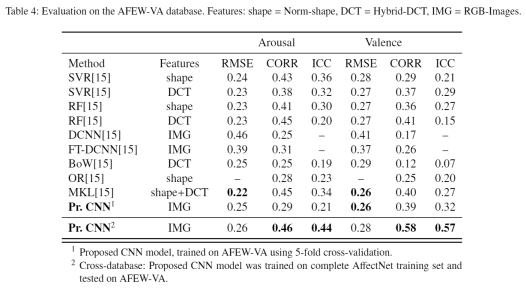
\includegraphics[angle=0, width=0.9\textwidth]{Figures/benchmark.PNG}
  \caption{Benchmark from the paper 'Simultaneous Prediction of Valence/Arousal and Emotions on AffectNet, Aff-Wild and AFEW-VA' \citep{Handrich:2020:SimultaneousPredVA}}
  \label{fig:BenchmarkOnAFEW-VA}
  \end{center}
\end{figure}

The proposed CNN approach by \citet{Handrich:2020:SimultaneousPredVA} outperformed the results of Neural Network based approaches (DCNN and FT-DCNN) by \citet{Kossaifi:2017:AFEW-VADatabase}. Only when comparing the results to the best performing algorithm, Multiple Kernel Learning (MKL), in terms of RMSE did it reveal a slightly higher loss.


%%%%%%%%%%%%%%%%%%%%%%%%%%%%%%%%%%%%%%%%%%%%%%%%%%%%%%%%%%%

\section{Results}
The results for the approach proposed in this Master thesis were achieved by shuffling data while making sure that training, validation and testing data stayed subject-independent. The following two graphs display the learning curves during training for the selected metrics, namely RMSE and CORR, for the predicted Valence values.

\begin{figure}[H]
  \centering
  \subfloat[Valence - RMSE]{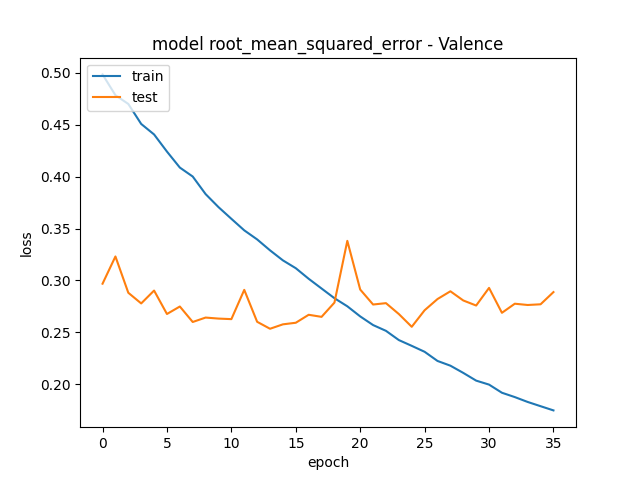
\includegraphics[width=0.5\textwidth]{Figures/rmse_out1.png}\label{fig:ValenceRMSE}}
  \hfill
  \subfloat[Valence - CORR]{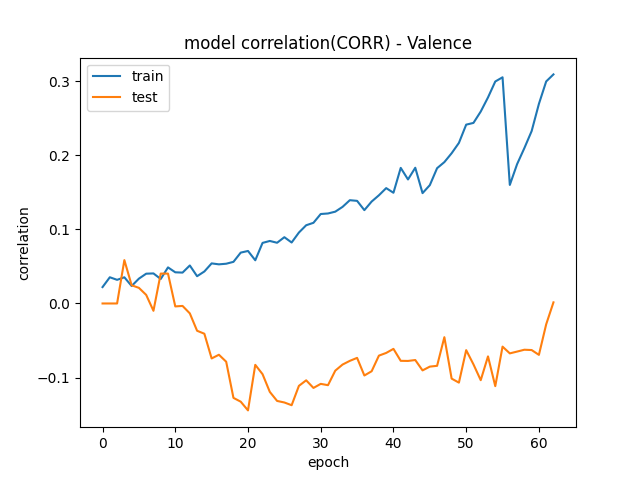
\includegraphics[width=0.5\textwidth]{Figures/correlation_out1.png}\label{fig:ValenceCORR}}
  \caption{Learning curves for Valence}
\end{figure}

\begin{figure}[H]
  \centering
  \subfloat[Arousal - RMSE]{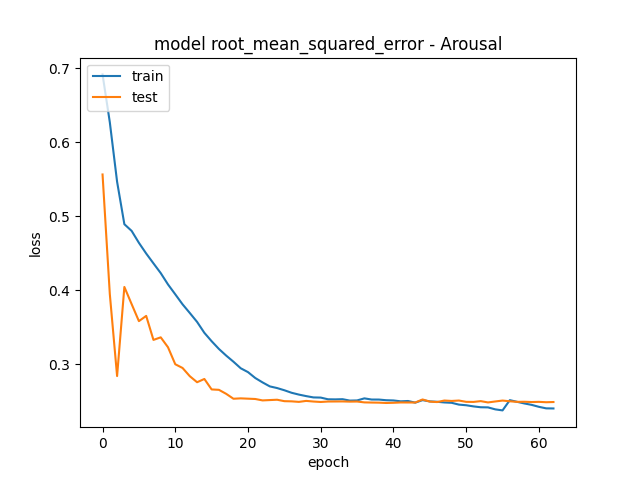
\includegraphics[width=0.5\textwidth]{Figures/rmse_out2.png}\label{fig:ArousalRMSE}}
  \hfill
  \subfloat[Arousal - CORR]{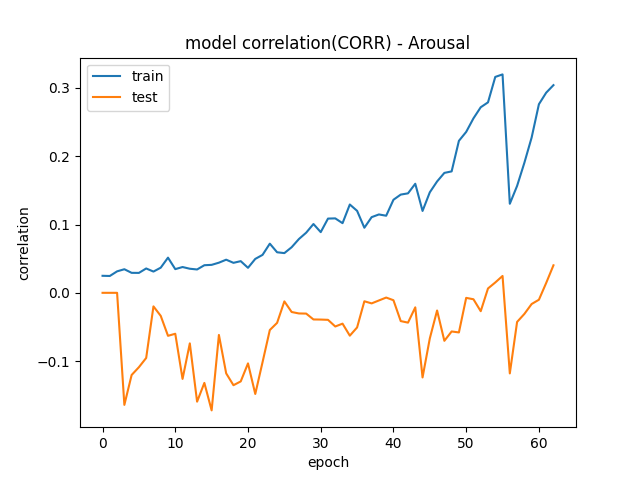
\includegraphics[width=0.5\textwidth]{Figures/correlation_out2.png}\label{fig:ArousalCORR}}
  \caption{Learning curves for Arousal}
\end{figure}

Theoretically, the ideal learning curve would show an exact match between the curves for training and testing/validation. In practice however, the goal is to minimize the difference between training and testing/validation curve over training time and stop training before they diverge from each other. This behavior can be seen for the RMSE metric for Valence and Arousal. The CORR metric instead diverged from each other for training and validation, which is a rather negative behavior.
\newline\newline
In summary, the learning curves can be regarded as rather positive, which is reinforced by achieved results presented in the following table. These were obtained through the implementation of the design choices presented in this Master's thesis with subject-independent data.

\begin{table}[H]
\begin{center}
\begin{tabular}{@{}rcccc@{}}
\toprule
\multicolumn{1}{c}{} & \begin{tabular}[c]{@{}c@{}}RMSE\\ Valence\end{tabular} & \begin{tabular}[c]{@{}c@{}}RMSE\\ Arousal\end{tabular} & \begin{tabular}[c]{@{}c@{}}CORR\\ Valence\end{tabular} & \begin{tabular}[c]{@{}c@{}}CORR\\ Arousal\end{tabular} \\ \midrule
\begin{tabular}[c]{@{}r@{}}best result\\ (without CV)\end{tabular} & 0.24 & 0.22 & 0.38 & 0.46 \\
\begin{tabular}[c]{@{}r@{}}best result\\ (with 5-fold-CV)\end{tabular} & 0.27 & 0.25 & 0.22 & 0.27 \\ \bottomrule
\end{tabular}
\caption{Results of the proposed approach}
\label{tab:Results}
\end{center}
\end{table}

The best result without Cross-Validation was achieved when not utilizing any Data Augmentation nor any landmarks. The best result with 5-fold-CV, on the other hand, was achieved with Data Augmentation and utilizing landmarks in the form of a heatmap overlay.

%%%%%%%%%%%%%%%%%%%%%%%%%%%%%%%%%%%%%%%%%%%%%%%%%%%%%%%%%%%%%
\section{Comparison}
The following table gives an overview of the results obtained by \citet{Kossaifi:2017:AFEW-VADatabase},  \citet{Handrich:2020:SimultaneousPredVA} as well as the approach taken by the researcher of this Master's thesis. All the results are directly comparable as they were achieved by performing 5-fold-cross-validation with subject independent data in between folds.

\begin{table}[H]
\begin{center}
\begin{tabular}{@{}ccccccc@{}}
\toprule
\rowcolor[HTML]{FCFF2F} 
\multicolumn{1}{l}{\cellcolor[HTML]{FCFF2F}} & \textbf{Method} & \textbf{Evaluation} & \textbf{\begin{tabular}[c]{@{}c@{}}RMSE\\ Valence\end{tabular}} & \textbf{\begin{tabular}[c]{@{}c@{}}RMSE\\ Arousal\end{tabular}} & \cellcolor[HTML]{FCFF2F}\textbf{\begin{tabular}[c]{@{}c@{}}CORR\\ Valence\end{tabular}} & \textbf{\begin{tabular}[c]{@{}c@{}}CORR\\ Arousal\end{tabular}} \\ \midrule
AFEW-VA & FT-DCNN & \begin{tabular}[c]{@{}c@{}}5-fold CV\\ subject indep.\end{tabular} & 0.37 & 0.39 & 0.26 & 0.31 \\
\begin{tabular}[c]{@{}c@{}}Simultaneous\\ VA prediction\end{tabular} & CNN & \begin{tabular}[c]{@{}c@{}}5-fold CV\\  subject indep.\end{tabular} & 0.26 & 0.25 & 0.39 & 0.29 \\
\textbf{\begin{tabular}[c]{@{}c@{}}RESULTS\\ THESIS\end{tabular}} & \begin{tabular}[c]{@{}c@{}}FT-DCNN\\ (VGGFace)\end{tabular} & \begin{tabular}[c]{@{}c@{}}5-fold CV\\ subject indep.\end{tabular} & 0.27 & 0.25 & 0.22 & 0.27 \\
\textbf{\begin{tabular}[c]{@{}c@{}}RESULTS\\ THESIS\end{tabular}} & \begin{tabular}[c]{@{}c@{}}FT-DCNN\\ (VGGFace)\end{tabular} & \begin{tabular}[c]{@{}c@{}}no CV\\ subject indep.\end{tabular} & 0.24 & 0.22 & 0.38 & 0.46 \\ \bottomrule
\end{tabular}
\caption{Comparison of final results}
\label{tab:ResultsComparison}
\end{center}
\end{table}

The results clearly show that the approach proposed in this Master thesis is substantially outperforming the results obtained by \citet{Kossaifi:2017:AFEW-VADatabase} in terms of Root-Mean-Squared-Error loss. It shows that RMSE is lower by 0.10 for valence and 0.14 for arousal, while the Correlation is lower by 0.04 for valence and 0.04 for arousal. In comparison to the approach proposed by \citet{Handrich:2020:SimultaneousPredVA} the results obtained by the researcher were pretty similar for the RMSE metric, but worse for the CORR with 0.17 lower for valence and 0.02 lower for arousal.
\newline\newline
In conclusion, it can be said that the results of this thesis are up to date with the state-of-the-art proposed by \citet{Handrich:2020:SimultaneousPredVA} in \citeyear{Handrich:2020:SimultaneousPredVA} for Emotion Recognition In-The-Wild with the AFEW-VA dataset \citep{Kossaifi:2017:AFEW-VADatabase}. The results also showed that fine-tuning a state-of-the-art pre-trained Neural Network is a very good way to go about beating current state-of-the-art Machine Learning challenges. It further showed that with further optimization, the proposed approach could even outperform the recent results from 2017.

\subsubsection{FaceReader application}
The FaceReader product of the company Noldus \citep{Noldus:2020:Facereader} is an application that is optimized for researchers to recognize emotions from facial expressions shown in videos. The product records the user and outputs categorical values for emotions, as well as Valence and Arousal. The initial goal was to compare the outcomes of this Master thesis with the analysis results of the FaceReader application.
\newline\newline
As confirmed through an sample experiment conducted by the researcher of this thesis, the FaceReader application failed to detect faces in every third frame due to imperfect conditions (e.g. a not-perfectly illuminated room). For this comparison no results can be presented as the approach for the FaceReader application is designed for laboratory conditions (they recommended the camera be placed slightly below eye-level, and that there be no shadow in the person's face). Therefore, their claimed accuracy (98 percent) cannot be compared to the In-The-Wild data utilized in this Master's thesis.
% However, as mentioned in the Quick Setup Guide, there approach is based upon the premise that the camera is placed slightly below eye-level of the test person and that good lightning, without shadow in the test person's face is crucial. Therefore, there claimed accuracy (from a phone call) with 98 percent cannot be compared to In-The-Wild data with imperfect conditions.
% Through a trial period the product was tested. As a camera an off-the-shelf integrated laptop camera was used in an weakly illuminated room. During the trial period the author realized, that the FaceReader often failed to provide information on expression intensity due to mostly not being able to find a face or also due to bad image quality. In total, in a 9 second experiment it was only able to detect the emotions during 3 of those 9 seconds.


%%%%%%%%%%%%%%%%%%%%%%%%%%%%%%%%%%%%%%%%%%%%%%%%%%%%%%%%%%%%%%%%
\section{Ablation Study}
This chapter is dedicated to the study of specific modules/design choices taken during the implementation. The chapter will be guided by the research paradigm of 'Ablation study'. Each study is comparing a selected base model with a modified model by leaving out a chosen feature. As a result of this comparison, valuable insights can be gained about the specific design choice or module. Furthermore, it needs to be pointed out that the below presented approaches are not in any chronological order, but are independent studies at different points in time during the writing of this Master's thesis.

%%%%%%%%%%%%%%%%%%%%%%%%%%%%%%%%%%%%%%%%%%%%%%%%%%%%%%%%%%%%%%%%
\subsection{Network architecture}
Both, the ResNet50 and VGG16 architecture are available for the pre-trained VGGFace and are very appreciated in the community. They have shown their qualities in the famous ImageNet competition with ResNet50 ending up winning the first price in 2015. ResNet50 is a deep neural network with 50 layers stacked upon each other and about 25 million parameters. Through their 'skip connection' concept their deep network is still able to train in deeper layers. VGG16 in comparison does not have as many layers, but is comprised of around 40 million parameters to be trained.
\newline\newline
ResNet50 was initially chosen due to it's deep layered approach and was compared to VGG16 in order to confirm its superiority in the challenge at hand. A comparison between both can be seen in the following table:

\hl{here table with results form ResNet50 vs. VGG16 (with DataAug + Standardization)}


%%%%%%%%%%%%%%%%%%%%%%%%%%%%%%%%%%%%%%%%%%%%%%%%%%%%%%%%%%%%%%%%
\subsection{MTCNN (Multi-task Cascaded Convolutional Neural Network)}
The MTCNN module is a pre-trained Neural Network that is used for detecting faces and determining its bounding box in an image/frame. Before talking about what difference the use of the MTCNN module makes towards the proposed solution, it is interesting to point out how often the module succeeds or fails to detect faces.
\newline\newline
During training with the AFEW-VA dataset, which consisted of 30.051 frames, the MTCNN module failed to detect the person's face in 961 cases. This represents 3.2 percent of all images, or a success rate of 96.8 percent.
% Out of 30051 frames it only failed to detect a face in 961 faces, this presents 3.2 percent of all images.
\newline\newline
The results were achieved with the use of the MTCNN module: faces inside an image were detected, the primary face was selcted, cut along its bounding box, and fed into the neural network. For images/frames were a face could not be detected, the original image was resized, and then fed into the NN.
\newline\newline
The results presented in the following table were achieved with the aforementioned methods and hyper parameters. The difference lay on the inclusion of the MTCNN module, on whether images were cropped to fit the person's face, or on whether the images got fed directly into the VGGFace model.

\begin{table}[H]
\begin{center}
\begin{tabular}{@{}rcccc@{}}
\toprule
\multicolumn{1}{c}{} & \begin{tabular}[c]{@{}c@{}}RMSE\\ Valence\end{tabular} & \begin{tabular}[c]{@{}c@{}}RMSE\\ Arousal\end{tabular} & \begin{tabular}[c]{@{}c@{}}CORR\\ Valence\end{tabular} & \begin{tabular}[c]{@{}c@{}}CORR\\ Arousal\end{tabular} \\ \midrule
with MTCNN & 0.24 & 0.24 & 0.13 & 0.15 \\
without MTCNN & 0.24 & 0.26 & -0.02 & 0.08 \\ \bottomrule
\end{tabular}
\caption{Experiment: MTCNN Module}
\label{tab:ExperimentMTCNN}
\end{center}
\end{table}

The results above can be clearly summarized as follows: The use of the MTCNN module for face detection + bounding boxing clearly contributed to the overall improvement of the model's performance. As the learning curves looked similar for both ways, it is not further illustrated here.
% \begin{figure}[H]
%   \centering
%   \subfloat[with MTCNN]{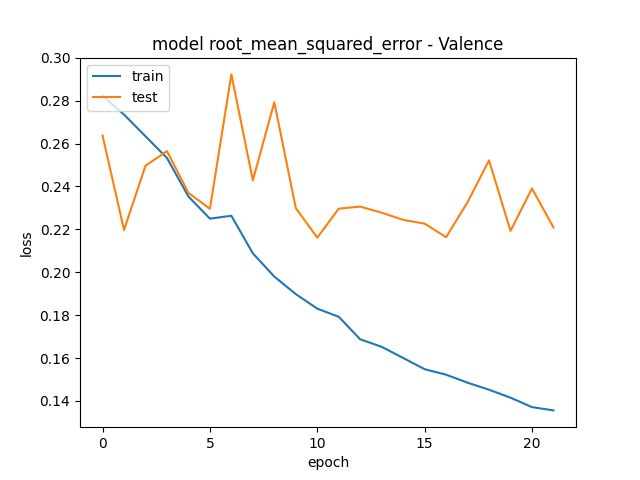
\includegraphics[width=0.5\textwidth]{Figures/mtcnn_val_rmse.png}\label{fig:MTCNNValRMSE}}
%   \hfill
%   \subfloat[without MTCNN]{\includegraphics[width=0.5\textwidth]{Figures/nomtcnn_val_rmse.png}\label{fig:NoMTCNNValRMSE}}
%   \caption{Comparison of learning curve for valence using the RMSE metric}
% \end{figure}
\newline\newline
As mentioned above, the MTCNN module failed to detect faces in about 3.2 percent of all images within this dataset. Whenever this happened, the original image was used as an input instead of feeding the cropped image containing the persons's face, into the Neural Network. This begs the question of whether this was truly the best approach, or whether it would have been better to discard those frames, so that the model can better focus on learning the specific facial features.
\newline\newline
This was done in an experiment: The performance of the model was compared with the original frame present, vis-a-vis the frame when the model couldn't detect a face. The results are summarized in the following table:

\begin{table}[H]
\begin{center}
\begin{tabular}{rcccc}
\hline
\multicolumn{1}{c}{} & \begin{tabular}[c]{@{}c@{}}RMSE\\ Valence\end{tabular} & \begin{tabular}[c]{@{}c@{}}RMSE\\ Arousal\end{tabular} & \begin{tabular}[c]{@{}c@{}}CORR\\ Valence\end{tabular} & \begin{tabular}[c]{@{}c@{}}CORR\\ Arousal\end{tabular} \\ \hline
keeping original frame & 0.26 & 0.25 & 0.15 & -0.05 \\
discarding frame & 0.27 & 0.25 & -0.11 & 0.14 \\ \hline
\end{tabular}
\caption{Experiment: Undetected Faces}
\label{tab:UndetectedFaces}
\end{center}
\end{table}

In summary, it can be said that there was a slight inclination towards keeping the original frame in terms of lower RMSE and higher CORR. However, the difference between those two approaches was so minor that it can be regarded as negligible.

%%%%%%%%%%%%%%%%%%%%%%%%%%%%%%%%%%%%%%%%%%%%%%%%%%%%%%%%%%%%%%%%
\subsection{Multi- Phase Fine-Tuning}
Multi-Phase Fine-Tuning is an approach aiming to increase the performance of a pre-trained neural network for a specific challenge at hand. While a conventional fine-tuning approach consists of unfreezing all the needed layers at once at the beginning of the training, the Multi-Phase Fine-Tuning involves the successive unfreezing of groups of layers. The neural network's to be updated weights were increased over several phases. As shown by \citet{Sarhan:2020:MultiPhaseFineTuning}, Multi-Phase Fine-Tuning resulted in higher classification accuracy while at the same time requiring less training time in comparison to earlier fine-tuning approaches.
% \begin{quote}
% In this paper, we propose multi-phase fine-tuning for tuning deep networks from typical object recognition to Sign Language Recognition (SLR). It extends the successful idea of transfer learning by fine-tuning the network’s weights over several phases. Starting from the top of the network, layers are trained in phases by successively unfreezing layers for training. We apply this novel training approach to SLR, since in this application, training data is scarce and differs considerably from the datasets which are usually used for pre-training. Our experiments show that multi-phase fine-tuning can reach significantly better accuracy in fewer training epochs compared to previous finetuning techniques
% Results show that compared to earlier fine-tuning approaches, multi-phase fine-tuning has a higher classification accuracy and requires less training time for this pair of domains.
% \citep[~p. 1]{Sarhan:2020:MultiPhaseFineTuning}
\newline\newline
The results achieved in this Master thesis can be seen in the 'Results' section. The following figure, a result of the Multi-Phase Fine-Tuning for the RMSE metric for 'Valence, provides a basis for the comparison between different fine-tuning approaches:

\begin{figure}[H]
  \begin{center}
  \includegraphics[angle=0, width=0.6\textwidth]{Figures/rmse_out1.png}
  \caption{Learning curve for Multi-Phased Fine-Tuning (FT) for RMSE of 'Valence'}
  \label{fig:MultiPhaseFT}
  \end{center}
\end{figure}

\begin{table}[H]
\begin{center}
\begin{tabular}{ccccc}
\hline
 & \begin{tabular}[c]{@{}c@{}}RMSE\\ Valence\end{tabular} & \begin{tabular}[c]{@{}c@{}}RMSE\\ Arousal\end{tabular} & \begin{tabular}[c]{@{}c@{}}CORR\\ Valence\end{tabular} & \begin{tabular}[c]{@{}c@{}}CORR\\ Arousal\end{tabular} \\ \hline
\multicolumn{1}{r}{\begin{tabular}[c]{@{}r@{}}base model\\ (without landmarks)\end{tabular}} & 0.24 & 0.22 & 0.38 & 0.46
\end{tabular}
\caption{Results for Multi-Phased Fine-Tuning (FT)}
\label{tab:MultiPhaseFT}
\end{center}
\end{table}

In contrast to the Multi-Phase Fine-Tuning, the Single-Phase Fine-Tuning approach was conducted. The number of final layers of the VGGFace model were gradually unfrozen. In figure \ref{fig:SinglePhaseFTall} all layers were unfrozen, and in figure \ref{fig:SinglePhaseFT70} the last 70 out of 175 layers of the model's architecture were unfrozen. The following figures showed the results obtained during training, for the selected two variants of Single-Phase Fine-Tuning strategies:

\begin{figure}[H]
  \centering
  \subfloat[Single-Phase FT with all layers trainable]{\includegraphics[width=0.5\textwidth]{Figures/rmse_out1_all.png}\label{fig:SinglePhaseFTall}}
  \hfill
  \subfloat[Single-Phase FT with 70 layers trainable]{\includegraphics[width=0.5\textwidth]{Figures/rmse_out1_70layers.png}\label{fig:SinglePhaseFT70}}
  \caption{Single-Phase Fine-Tuning results for the RMSE metric of 'Valence'}
\end{figure}

\begin{table}[H]
\begin{center}
\begin{tabular}{@{}rcccc@{}}
\toprule
\multicolumn{1}{c}{} & \begin{tabular}[c]{@{}c@{}}RMSE\\ Valence\end{tabular} & \begin{tabular}[c]{@{}c@{}}RMSE\\ Arousal\end{tabular} & \begin{tabular}[c]{@{}c@{}}CORR\\ Valence\end{tabular} & \begin{tabular}[c]{@{}c@{}}CORR\\ Arousal\end{tabular} \\ \midrule
\begin{tabular}[c]{@{}r@{}}Single-Phase FT\\ (all layers trainable)\end{tabular} & 0.24 & 0.24 & 0.13 & 0.15 \\
\begin{tabular}[c]{@{}r@{}}Single-Phase FT\\ (70 layers trainable)\end{tabular} & 0.21 & 0.26 & 0.05 & -0.08 \\ \bottomrule
\end{tabular}
\caption{Single-Phased Fine-Tuning (FT) comparison: layers trainable}
\label{tab:SPFTLayersTrainable}
\end{center}
\end{table}

It can clearly be seen in both figures above that the progress of the 'test' curve isn't showing a downward trend, as one might have expected, and have seen in figure \ref{fig:MultiPhaseFT}. This behavior is a strong indication that the neural network is not able to generalize well from its training, and is thus overfitting.
\newline\newline
Comparing the figures \ref{fig:SinglePhaseFTall} and \ref{fig:SinglePhaseFT70} with their respective results in table \ref{tab:SPFTLayersTrainable}, one can observe that fine-tuning only subset of layers yields better results in terms of a low RMSE error. However, for both approaches, the 'test' curve displays a rather erratic behavior in comparison to the smooth 'test' curve in figure \ref{fig:MultiPhaseFT}. 
\newline\newline
The above presented observation on overfitting raises the question: How many layers should be unfrozen to achieve the best possible result? \newline
Here, the Multi-Phase Fine-Tuning approach came in handy. Experiments performed with the Multi-Phase FT approach showed that a higher step size generally resulted in a higher loss. Even while all the other parameters stayed the same, the step size can have an enormous impact on the model performance. The following table details the results of a model with a step size of 1, compared to a model with a step size of 2:

\begin{figure}[H]
  \centering
  \subfloat[Multi-Phase FT with step size 1]{\includegraphics[width=0.5\textwidth]{Figures/multi_phase_step1.png}\label{fig:MultiPhaseStep1}}
  \hfill
  \subfloat[Multi-Phase FT with step size 2]{\includegraphics[width=0.5\textwidth]{Figures/multi_phase_step2.png}\label{fig:MultiPhaseStep2}}
  \caption{Multi-Phase Fine-Tuning results for the RMSE metric of 'Valence'}
\end{figure}

\begin{table}[H]
\begin{center}
\begin{tabular}{@{}rcccc@{}}
\toprule
\multicolumn{1}{c}{} & \begin{tabular}[c]{@{}c@{}}RMSE\\ Valence\end{tabular} & \begin{tabular}[c]{@{}c@{}}RMSE\\ Arousal\end{tabular} & \begin{tabular}[c]{@{}c@{}}CORR\\ Valence\end{tabular} & \begin{tabular}[c]{@{}c@{}}CORR\\ Arousal\end{tabular} \\ \midrule
\begin{tabular}[c]{@{}r@{}}base model\\ (step\_size=2)\end{tabular} & 0.24 & 0.22 & 0.38 & 0.46 \\
\begin{tabular}[c]{@{}r@{}}MP-FT alt\\ (step\_size=1)\end{tabular} & 0.20 & 0.19 & 0.07 & 0.13 \\ \bottomrule
\end{tabular}
\caption{Multi-Phased Fine-Tuning (FT) comparison: step size}
\label{tab:FTStepSize}
\end{center}
\end{table}

The results show that step size 2 prevails over the results for step size 1 in this model architecture. Furthermore, when observing the respective figures, it can be seen that the 'test' curve for figure \ref{fig:MultiPhaseStep1} initially increased in loss, and only decreased more sharply after about 20 epochs. At the same time, figure \ref{fig:MultiPhaseStep2} decreased sharply in the beginning and flattened out, which indicates a higher potential for better performance after some optimization/tweaking.
\newline\newline
In terms of numerical results, step size 1 is performed better in terms of RMSE loss. However, adding the element of the Pearson correlation (CORR), using step size 2 clearly exhibited better results.


%%%%%%%%%%%%%%%%%%%%%%%%%%%%%%%%%%%%%%%%%%%%%%%%%%%%%%%%%%%%%%%%
\subsection{Data Augmentation}


\begin{figure}[H]
  \centering
  \subfloat[Without Data Augmentation 1]{\includegraphics[width=0.5\textwidth]{Figures/rmse_out1_noDataAug.png}\label{fig:NoDataAug}}
  \hfill
  \subfloat[With Data Augmenation]{\includegraphics[width=0.5\textwidth]{Figures/rmse_out1_wDataAug.png}\label{fig:WithDataAug}}
  \caption{Comparison of the Data Augmentation module for the RMSE metric of 'Valence'}
\end{figure}


% Please add the following required packages to your document preamble:
% \usepackage{booktabs}
\begin{table}[H]
\begin{center}
\begin{tabular}{@{}rcccc@{}}
\toprule
\multicolumn{1}{c}{} & \begin{tabular}[c]{@{}c@{}}RMSE\\ Valence\end{tabular} & \begin{tabular}[c]{@{}c@{}}RMSE\\ Arousal\end{tabular} & \begin{tabular}[c]{@{}c@{}}CORR\\ Valence\end{tabular} & \begin{tabular}[c]{@{}c@{}}CORR\\ Arousal\end{tabular} \\ \midrule
\begin{tabular}[c]{@{}r@{}}Multi-Phase FT\\ (without Data Aug.)\end{tabular} & 0.29 & 0.25 & -0.10 & 0.12 \\
\begin{tabular}[c]{@{}r@{}}Multi-Phase FT\\ (with Data Aug.)\end{tabular} & 0.26 & 0.26 & 0.15 & -0.05
\end{tabular}
\caption{Multi-Phased Fine-Tuning (FT) comparison: Data Augmentation}
\label{tab:MPFTDataAug}
\end{center}
\end{table}



%%%%%%%%%%%%%%%%%%%%%%%%%%%%%%%%%%%%%%%%%%%%%%%%%%%%%%%%%%%%%%%%
\subsection{Regularization}
Regularization techniques are generally used to introduce error and/or randomness during the training process which makes training for the model harder, but the hope is that they also provide better generalization capabilities. Better generalization capabilities result in a better performance during validation/testing of the model, and a reduction in overfitting. The experiments presented in this section are being compared to the presented model above (i.e., Multi-Phased FT without Data Augmentation).

\textbf{Dropout}\newline
Based on the illustrated outcomes above, an ablation study was conducted by eliminating the Dropout layers from the model architecture. The achieved results for the RMSE metric of 'Valence' can be seen below:

\begin{figure}[H]
  \begin{center}
  \includegraphics[angle=0, width=0.6\textwidth]{Figures/rmse_out1_noDropout.png}
  \caption{Learning curve for RMSE metric of 'Valence' without any Dropout}
  \label{fig:AblationNoDropout}
  \end{center}
\end{figure}

As expected, due to the missing regularization effect of the Dropout layers, the results achieved during training showcased a much higher validation/testing loss in comparison to the training loss. Moreover, the results compared to the base model, Multi-Phased FT without Data Augmentation performed equally bad without any Dropout:

\begin{table}[H]
\begin{center}
\begin{tabular}{@{}rcccc@{}}
\toprule
\multicolumn{1}{c}{} & \begin{tabular}[c]{@{}c@{}}RMSE\\ Valence\end{tabular} & \begin{tabular}[c]{@{}c@{}}RMSE\\ Arousal\end{tabular} & \begin{tabular}[c]{@{}c@{}}CORR\\ Valence\end{tabular} & \begin{tabular}[c]{@{}c@{}}CORR\\ Arousal\end{tabular} \\ \midrule
\begin{tabular}[c]{@{}r@{}}Multi-Phased FT\\ (no Data Aug.)\end{tabular} & 0.29 & 0.25 & -0.10 & 0.12 \\
\begin{tabular}[c]{@{}r@{}}Multi-Phased FT\\ without Dropout\end{tabular} & 0.47 & 0.49 & -0.11 & 0.03
\end{tabular}
\caption{Multi-Phased Fine-Tuning (FT) comparison: Dropout}
\label{tab:MPFTDropout}
\end{center}
\end{table}

\textbf{Batch Normalization}\newline
The same ablation approach was conducted for Batch Normalization while keeping all the other parameters the same. This signified that it was based upon the same architecture as above described, including the Dropout layer, but without the Batch Normalization layer. The result in terms of the RMSE metric for 'Valence' looks like this:

\begin{figure}[H]
  \begin{center}
  \includegraphics[angle=0, width=0.6\textwidth]{Figures/rmse_out1_noBatchNorm.png}
  \caption{Learning curve for RMSE metric of 'Valence' without any Batch Normalization}
  \label{fig:AblationNoBatchNorm}
  \end{center}
\end{figure}         

Even after the Batch Normalization layer was removed, the model barely improved in terms of its training loss during training compared to the ablation of Dropout. An additional negative behavior was that the curve for the test loss was very volatile/erratic and even increased. This results in the following outcomes for the evaluation of this ablation:

\begin{table}[H]
\begin{center}
\begin{tabular}{@{}rcccc@{}}
\toprule
\multicolumn{1}{c}{} & \begin{tabular}[c]{@{}c@{}}RMSE\\ Valence\end{tabular} & \begin{tabular}[c]{@{}c@{}}RMSE\\ Arousal\end{tabular} & \begin{tabular}[c]{@{}c@{}}CORR\\ Valence\end{tabular} & \begin{tabular}[c]{@{}c@{}}CORR\\ Arousal\end{tabular} \\ \midrule
\begin{tabular}[c]{@{}r@{}}Multi-Phased FT\\ (no Data Aug.)\end{tabular} & 0.29 & 0.25 & -0.10 & 0.12 \\
\begin{tabular}[c]{@{}r@{}}Multi-Phased FT\\ without BatchNorm\end{tabular} & 0.50 & 0.69 & -0.08 & 0.00
\end{tabular}
\caption{Multi-Phased Fine-Tuning (FT) comparison: Batch Normalization}
\label{tab:MPFTNoBatchNorm}
\end{center}
\end{table}

\textbf{L2 regularization}\newline
Even though L2 regularization was not included in the proposed model architecture, there were multiple experiments to explore the benefit of L1/L2 regularization during the fine-tuning process. However, all these efforts turned out to lower the performance of the model overall. In order to explain why this regularization technique was not helpful, an illustration and discussion of two approaches will be discussed through the two figures below. The first figure illustrates the results of applying L2 regularization to the single Dense layer at the top of the model.

\begin{figure}[H]
  \begin{center}
  \includegraphics[angle=0, width=0.6\textwidth]{Figures/rmse_out1_L2Dense.png}
  \caption{Learning curve for RMSE metric of 'Valence' with L2 regularization for the Dense layer}
  \label{fig:AblationL2Dense}
  \end{center}
\end{figure}

As it can be seen from the graph above, the application of L2 regularization to the Dense layer performed initially well on the validation/test data, like in the base model. However, toward later epochs, the validation/test loss started to increase which likely indicates overfitting of the model. The results for this approach can be summarized as follows:

\begin{table}[H]
\begin{center}
\begin{tabular}{@{}rcccc@{}}
\toprule
\multicolumn{1}{c}{} & \begin{tabular}[c]{@{}c@{}}RMSE\\ Valence\end{tabular} & \begin{tabular}[c]{@{}c@{}}RMSE\\ Arousal\end{tabular} & \begin{tabular}[c]{@{}c@{}}CORR\\ Valence\end{tabular} & \begin{tabular}[c]{@{}c@{}}CORR\\ Arousal\end{tabular} \\ \midrule
\begin{tabular}[c]{@{}r@{}}Multi-Phased FT\\ (no Data Aug.)\end{tabular} & 0.29 & 0.25 & -0.10 & 0.12 \\
\begin{tabular}[c]{@{}r@{}}Multi-Phased FT\\ L2-Reg. Dense Layer\end{tabular} & 0.28 & 0.25 & -0.10 & 0.13
\end{tabular}
\caption{Multi-Phased Fine-Tuning (FT) comparison: L2-Regularization for Dense Layer}
\label{tab:MPFTL2RegDense}
\end{center}
\end{table}

Surprisingly, this approach behaved slightly better than the base model. However, the improvement is so marginal that it can be regarded as not having any influence on the model performance.
\newline\newline
Another promising approach was the application of L2 regularization to all trainable (=unfrozen) layers from the pretrained VGGFace network, without applying it to the model's Dense layer. The results achieved for a 0.01 regularizer for the RMSE metric, for 'Valence' look like this:

\begin{figure}[H]
  \begin{center}
  \includegraphics[angle=0, width=0.6\textwidth]{Figures/rmse_out1_L2VGGFace.png}
  \caption{Learning curve for RMSE metric of 'Valence' with L2 regularizer for the unfrozen layers in VGGFace}
  \label{fig:AblationL2VGGFace}
  \end{center}
\end{figure}

The curve, especially from the 90th epoch on, looks quite promising in terms of validation/test loss. However, the actual results obtained during the evaluation of the model on a separate test set showed substantially lower numbers for RMSE. The results are summarized and compared in the table below.

\begin{table}[H]
\begin{center}
\begin{tabular}{@{}rcccc@{}}
\toprule
\multicolumn{1}{c}{} & \begin{tabular}[c]{@{}c@{}}RMSE\\ Valence\end{tabular} & \begin{tabular}[c]{@{}c@{}}RMSE\\ Arousal\end{tabular} & \begin{tabular}[c]{@{}c@{}}CORR\\ Valence\end{tabular} & \begin{tabular}[c]{@{}c@{}}CORR\\ Arousal\end{tabular} \\ \midrule
\begin{tabular}[c]{@{}r@{}}Multi-Phased FT\\ (no Data Aug.)\end{tabular} & 0.29 & 0.25 & -0.10 & 0.12 \\
\begin{tabular}[c]{@{}r@{}}Multi-Phased FT\\ L2-Reg. VGG Layer\end{tabular} & 0.40 & 0.28 & -0.07 & 0.03
\end{tabular}
\caption{Multi-Phased Fine-Tuning (FT) comparison: L2-Regularization for trainable VGGFace layers}
\label{tab:MPFTL2RegVGG}
\end{center}
\end{table}

In summary, it could be proven that various regularization techniques, such as Dropout and Batch Normalization improved the proposed model's generalization capabilities. However, in the case of applying L2 weight regularization to either Dense or pre-trained Convolutional layers, there was no substantial performance gain. On the contrary, it increased the validation, as well as the testing loss for both Valence and Arousal.
% Validation loss during training is lower than the training loss, which is very likely because of the reason that regularization was applied. This L2 regularization is only applied during training, but not validation/testing, which explains the significant difference between those values.
% https://www.pyimagesearch.com/2019/10/14/why-is-my-validation-loss-lower-than-my-training-loss/

%%%%%%%%%%%%%%%%%%%%%%%%%%%%%%%%%%%%%%%%%%%%%%%%%%%%%%%%%%%%%%%%
\subsection{Recurrent Neural Network}
% \textbf{- Can an LSTM capture the time-spatio changes between frames and thus enhance the performance of \gls{ER}}
% Data needs to be non-shuffled in order to do that
% -> Performance didn't increase

The idea behind applying a Recurrent Neural Network (RNNs) is to capture the time-spatial changes in between frames with the goal of further enhancing the performance of Emotion Recognition. The specific type of RNN applied is callled LSTM. Additionally, the model's architecture needed to be changed in order to allow for an input of sequences with 5 frames each. These are fed into the model and processed simultaneously, going through the CNN, then the LSTM layer and finally the classifier. Moreover, frames inside the dataset mustn't be shuffled in order to be able to capture time-spatial changes.
\newline\newline
Results achieved in terms of RMSE metric of 'Valence' with an LSTM layer look like this:

\begin{figure}[H]
  \begin{center}
  \includegraphics[angle=0, width=0.6\textwidth]{Figures/rmse_out_LSTM.png}
  \caption{Learning curve for RMSE metric of 'Valence' with LSTM}
  \label{fig:AblationLSTM}
  \end{center}
\end{figure}

The following table compares the base model, with a CNN only architecture, to the proposed CNN + LSTM architecture. It shows that the LSTM performs better in terms of RMSE, but lacks in CORR, which makes it hard to judge whether it is really a better choice as CORR usually indicates the models' generalization ability. 

\begin{table}[H]
\begin{center}
\begin{tabular}{rcc}
\hline
\multicolumn{1}{c}{Ablation study} & RMSE & CORR \\ \hline
\begin{tabular}[c]{@{}r@{}}base model\\ (CNN only)\end{tabular} & 0.46 & 0.42 \\
\begin{tabular}[c]{@{}r@{}}CNN + LSTM\\ (step size 3)\end{tabular} & 0.21 & 0.14 \\ \hline
\end{tabular}
\caption{Experiment: Prediction with and without LSTM}
\label{tab:LSTM}
\end{center}
\end{table}






%%%%%%%%%%%%%%%%%%%%%%%%%%%%%%%%%%%%%%%%%%%%%%%%%%%%%%%%%%%%%%%%
\subsection{Facial Landmarks}
The recognition of landmarks and its usage as a feature for increasing the performance of Emotion Recognition is well accepted in the scientific community. These landmarks are generally applied as an overlay to the original image and put through the Convolutional layers of the model architecture.
\newline\newline
Active Appearance Model is an approach that is considered as one of the most accurate approaches to detect landmarks of a person's face. It is described by \citet{Gao:2010:ActiveAppearanceModels} as very suitable for the extraction of compact features in various application. However, they admit that this approach can't satisfy real-time requirements sufficiently, due to its time consuming fitting process.
\newline\newline
This consideration led to the decision of implementing a fast performing algorithm for the task of landmark prediction, instead of an Active Appearance Model which needs for each face a few seconds to be fitted. The decision fell on the algorithm of 'Ensemble of Regression Trees(ERT)' \citep{Kazemi:2014:ShapePredictor} implemented as a pre-trained shape predictor by the dlib library, which predicts 68 facial landmarks. The outcome looks like this:

\begin{figure}[H]
  \begin{center}
  \includegraphics[angle=0, width=0.4\textwidth]{Figures/landmarks_as_dots.png}
  \caption{Landmarks as dots with dlib shape predictor}
  \label{fig:LandmarkdsDots}
  \end{center}
\end{figure}

According to the authors paper with the title 'One Millisecond Face Alignment with an Ensemble of Regression Trees' \citep{Kazemi:2014:ShapePredictor} the approach is able to predict 68 facial landmarks in real-time. The results of this approach are illustrated through the following figure and table:

\begin{figure}[H]
  \begin{center}
  \includegraphics[angle=0, width=0.6\textwidth]{Figures/rmse_out1_landmarks.png}
  \caption{Learning curve for RMSE metric of 'Valence' for Landmarks}
  \label{fig:ASM}
  \end{center}
\end{figure}

\begin{table}[H]
\begin{center}
\begin{tabular}{rcccc}
\hline
\multicolumn{1}{c}{Ablation study} & \begin{tabular}[c]{@{}c@{}}RMSE\\ Valence\end{tabular} & \begin{tabular}[c]{@{}c@{}}RMSE\\ Arousal\end{tabular} & \begin{tabular}[c]{@{}c@{}}CORR\\ Valence\end{tabular} & \begin{tabular}[c]{@{}c@{}}CORR\\ Arousal\end{tabular} \\ \hline
\begin{tabular}[c]{@{}r@{}}base model\\ (without landmarks)\end{tabular} & 0.24 & 0.22 & 0.38 & 0.46 \\
\begin{tabular}[c]{@{}r@{}}Landmarks\\ (with 68 data points)\end{tabular} & 0.21 & 0.22 & 0.02 & 0.00 \\ \hline
\end{tabular}
\caption{Experiment: Landmarks}
\label{tab:Landmarks}
\end{center}
\end{table}

The results show that the RMSE value slightly improves (decreases), while the CORR metric massively forfeits its positive correlation. This might indicate, that using landmarks for the recognition of emotions with the pre-trained VGGFace network is not a good fit.

% \textbf{- How much longer does the program need to run through for one image with an AAM?}

% Construction of landmarks for the whole dataset of 30051 images. From 7402 images it could not detect the face (with dlib face detector)

% The 'default' face detector from dlib fails to detect 7402 out of 30051 images, while the MTCNN only fails in 961 images to detect a face. => A logical conclusion would be to use MTCNN to detect the face and the respective bounding box while using the dlib shape predictor, based upon the ERT approach, to time-efficiently detect  facial landmarks.


%%%%%%%%%%%%%%%%%%%%%%%%%%%%%%%%%%%%%%%%%%%%%%%%%%%%%%%%%%%%%%%%
\subsubsection{Facial Landmarks as Heatmap}
Even though it could not be proven that facial landmarks improve the model performance, a consideration was to upgrade the landmark dots to a heatmap version. The observed learning curves and results obtained might exhibit further indications for the performance of utilizing facial landmarks. The outcome of applying a heatmap looks like this:

\begin{figure}[H]
  \begin{center}
  \includegraphics[angle=0, width=0.4\textwidth]{Figures/landmarks_as_heatmap.png}
  \caption{Landmarks as heatmap}
  \label{fig:LandmarksHeatmap}
  \end{center}
\end{figure}

The learning curve and results obtained can be observed in the following figure and table:

\begin{figure}[H]
  \begin{center}
  \includegraphics[angle=0, width=0.6\textwidth]{Figures/rmse_out1_heatmap.png}
  \caption{Learning curve for RMSE metric of 'Valence' for Active Shape Model with Heatmap}
  \label{fig:ASMHeatmap}
  \end{center}
\end{figure}

\begin{table}[H]
\begin{center}
\begin{tabular}{rcccc}
\hline
\multicolumn{1}{c}{Ablation study} & \begin{tabular}[c]{@{}c@{}}RMSE\\ Valence\end{tabular} & \begin{tabular}[c]{@{}c@{}}RMSE\\ Arousal\end{tabular} & \begin{tabular}[c]{@{}c@{}}CORR\\ Valence\end{tabular} & \begin{tabular}[c]{@{}c@{}}CORR\\ Arousal\end{tabular} \\ \hline
\begin{tabular}[c]{@{}r@{}}base model\\ (without landmarks)\end{tabular} & 0.24 & 0.22 & 0.38 & 0.46 \\
\begin{tabular}[c]{@{}r@{}}Heatmap\\ (from ASM)\end{tabular} & 0.22 & 0.22 & 0.00 & 0.00 \\ \hline
\end{tabular}
\caption{Experiment: ASMHeatmap}
\label{tab:ASMHeatmap}
\end{center}
\end{table}

Contrary, to the expectation of improving the model performance, using a heatmap instead of solely dots as an overlay slightly increases the RMSE and slightly decreases CORR. A possible explanation might be that the model has more difficulty extracting facial features because of the heatmap overlay. This overlay is drawing stepwise colored dots for the facial landmarks while putting a shadow over the residual parts of the image. This shadow might actually end up worsening the model performance.

%%%%%%%%%%%%%%%%%%%%%%%%%%%%%%%%%%%%%%%%%%%%%%%%%%%%%%%%%%%%%%%%
\subsubsection{Facial Landmarks as a Soft Attention overlay}
Due to the poor results from the before mentioned approaches, it was suspected, that the facial landmarks overlay in the form of dots or an heatmap is covering parts of the face that contain very important information for the detection of facial expressions. In order to prove/disprove this assumption, the facial landmarks overlay containing the dots was given a low opacity of 0.2. 

\begin{figure}[H]
  \begin{center}
  \includegraphics[angle=0, width=0.4\textwidth]{Figures/landmarks_as_softOverlay.png}
  \caption{Landmarks as a soft overlay}
  \label{fig:LandmarksSoftOverlay}
  \end{center}
\end{figure}

This approach is expected to preserve information about facial expressions in the image, while landmarks are illustrated with a coloured shadow at the respective landmark locations. Achieved results did indeed prove this suspicion that information got covered in previous methods. Thus, this approach performed significantly better as the heatmap approach. This can be seen in the following table:

\begin{figure}[H]
  \begin{center}
  \includegraphics[angle=0, width=0.6\textwidth]{Figures/rmse_out1_softAttention.png}
  \caption{Learning curve for RMSE metric of 'Valence' for Active Shape Model with Soft Attention landmarks}
  \label{fig:LandmarksSoftAttention}
  \end{center}
\end{figure}

\begin{table}[H]
\begin{center}
\begin{tabular}{@{}rcccc@{}}
\toprule
\multicolumn{1}{c}{Ablation study} & \begin{tabular}[c]{@{}c@{}}RMSE\\ Valence\end{tabular} & \begin{tabular}[c]{@{}c@{}}RMSE\\ Arousal\end{tabular} & \begin{tabular}[c]{@{}c@{}}CORR\\ Valence\end{tabular} & \begin{tabular}[c]{@{}c@{}}CORR\\ Arousal\end{tabular} \\ \midrule
\begin{tabular}[c]{@{}r@{}}base model\\ (without landmarks)\end{tabular} & 0.24 & 0.22 & 0.38 & 0.46 \\
\begin{tabular}[c]{@{}r@{}}Heatmap\\ (from ASM)\end{tabular} & 0.22 & 0.22 & 0.00 & 0.00 \\
\begin{tabular}[c]{@{}r@{}}Soft Attention Overlay\\ (from ASM)\end{tabular} & 0.19 & 0.20 & 0.08 & 0.07 \\ \bottomrule
\end{tabular}
\caption{Experiment: ASMSoftAttention}
\label{tab:ASMSoftAttention}
\end{center}
\end{table}

These results let the researcher conclude, that a direct overlay of landmarks on top of the image is detrimental to the generalization ability of the model. It is suspected, that the application of the landmarks on top of the image covers important information in the image and hinders the model to learn these features. Therefore, in order to utilize facial landmarks without hindering the learning ability of the model, landmarks will be kept in a separate mask, that is fed separately into the Neural Network.

\subsubsection{Facial Landmarks as separate mask}
Based on the aforementioned insight from the experiments with utilizing landmarks as an overlay on the image, it was concluded that landmarks cover important information in the image. Therefore, in this part landmarks were kept in a separate mask with pixel values ranging from 0 to +1. The constructed landmarks mask for the example can be seen in the following figure:

\begin{figure}[H]
  \begin{center}
  \includegraphics[angle=0, width=0.4\textwidth]{Figures/landmarks_as_heatmap_in_mask.png}
  \caption{Landmarks as a heatmap in mask}
  \label{fig:LandmarksMask}
  \end{center}
\end{figure}

This mask with its dimensions of 224x224 is then fed as an additional fourth channel to the respective RGB image. The output shape of this concatenation will be 224x224x4 and is repeated for each image in the training, validation and test dataset.
\newline\newline
As this image, due to its fourth channel doesn't fit anymore the input shape requirements for the pre-trained VGGFace network, a custom Neural Network had to be constructed and trained. In order to keep the outcomes comparable it was chosen to implement a ResNet50 architecture from scratch that takes a four channel image as input and consists of the same layers as the proposed architecture. The training results achieved with a Cyclic Learning Rate can be seen in the following table:

\begin{table}[H]
\begin{center}
\begin{tabular}{@{}rcccc@{}}
\toprule
\multicolumn{1}{c}{Ablation study} & \begin{tabular}[c]{@{}c@{}}RMSE\\ Valence\end{tabular} & \begin{tabular}[c]{@{}c@{}}RMSE\\ Arousal\end{tabular} & \begin{tabular}[c]{@{}c@{}}CORR\\ Valence\end{tabular} & \begin{tabular}[c]{@{}c@{}}CORR\\ Arousal\end{tabular} \\ \midrule
\begin{tabular}[c]{@{}r@{}}base model\\ (without landmarks)\end{tabular} & 0.24 & 0.22 & 0.38 & 0.46 \\
\begin{tabular}[c]{@{}r@{}}Soft Attention Overlay\\ (from ASM)\end{tabular} & 0.19 & 0.20 & 0.08 & 0.07 \\
\begin{tabular}[c]{@{}r@{}}Landmarks Mask\\ (from ASM)\end{tabular} & 0.24 & 0.24 & 0.10 & 0.20 \\ \bottomrule
\end{tabular}
\caption{Experiment: ASMLandmarksMask}
\label{tab:ASMLandmarksMask}
\end{center}
\end{table}

The results visibly show that this approach outperforms the previous landmark approaches, with the best being the 'Soft Attention' approach. Nevertheless, it still can not beat the results of the 'base model' based on not utilizing any landmarks at all. As a result, it can be said that the conducted experiments coul not prove that utilizing facial landmarks improves Emotion Recognition outcomes.  


%%%%%%%%%%%%%%%%%%%%%%%%%%%%%%%%%%%%%%%%%%%%%%%%%%%%%%%%%%%%%%%%
% \subsection{Landmarks with AAM (Active Appearance Model)}
% \textbf{Comparison ASM vs. AAM}
% - considerations run-time per image/batch
% - validation/testing loss improvement



\chapter{Application}
For PPI AG, the goal is to use the research conducted during this Master thesis as a scientific basis for a future application of this technology in one of their own business use cases. Therefore, this chapter will assess, whether Emotion Recognition is a viable assistance for consultants, as well as customers in the selected use case of video-call consultations.
\newline\newline
Firstly, a prototype was developed to prove that Emotion Recognition is a viable option for real-time predictions from a webcam stream.
\newline\newline
Secondly, a more meaningful interpretation of emotions was needed to provide consultants or customers with a more actionable metric. Interest was chosen to be the metric used to identify a customer's intention. Thus, an user experiment was conducted that compares the predicted interest based on emotions recognized from facial expressions with the stated level of interest by participants.

%%%%%%%%%%%%%%%%%%%%%%%%%%%%%%%%%%%%%%%%%%%%%%%%%%%%%%%%%%%%
\section{Prototype}
The first prototype was constructed as a local application that takes its video input from the PC's webcam. When the user presses the 'SPACE' key, the programm extracts the current frame of the video stream, detects the human face, recognizes its emotion in terms of valence and arousal, and prints the results onto the screen. A snapshot of this is provided in the following figure \ref{fig:PrototypeRealTime}. 

\begin{figure}[H]
  \begin{center}
  \includegraphics[angle=0, width=0.8\textwidth]{Figures/webcam_foto.PNG}
  \caption{Prototype application for real-time demonstration}
  \label{fig:PrototypeRealTime}
  \end{center}
\end{figure}

\textbf{Landmarks}\newline
It was from special interest to PPI AG whether such an approach would be suitable for real-time usage, especially in regards to utilizing landmarks. 
\newline\newline
A small test of 10 probes indicated that it took on average 0.7 seconds to perform Emotion Recognition without any landmarks in production. In comparison to that, additionally detecting landmarks and feeding them into the model did not result in any delay, as its performance was also on average 0.7 seconds. Such a low number, with less than 1 second, proves that this approach is definitely suitable for real-time use cases. 
\newline\newline
However, it needs to be pointed out that this could only be achieved with the dlib shape predictor, unlike an Active Appearance Model which would likely need more time to be constructed. Furthermore, it is to be expected that the average duration of 0.7 seconds further decreases when taking into account that the prediction be performed on a powerful server with GPU support instead of a laptop computer.

%%%%%%%%%%%%%%%%%%%%%%%%%%%%%%%%%%%%%%%%%%%%%%%%%%%%%%%%%%%%
\section{User Experiment (Interest)}
The experiment provided further insights into the utilization of Emotion Recognition for the identification of human interest. Thus, the goal was to be able to draw conclusions about the suspected correlation between recognized emotions and human interest. Before diving into the design and outcomes of the experiment, an identification approach of interest had to be created based upon current literature.
\newline\newline
There herein presented approach for identifying interest was based on the ideas from two different scientific contributions:
\begin{itemize}
    \item \citet{Kamaruddin:2016:MeasuringCustomerSatisfaction} determined a level of interest/appreciation by measuring how positive or negative an emotion (= valence) experience was on average.
    \item \citet{Poirier:2016:AdsFacialExpression} measured the effectiveness of ads by analyzing facial expressions. They claimed that the emotional journey is the strongest predictor of ad appreciation which is why they focused on the curve/profile created by the predicted emotion values for valence.
\end{itemize}

% \citet{Poirier:2016:AdsFacialExpression} measured the effectiveness of ads by analyzing facial expressions. \citet{Poirier:2016:AdsFacialExpression} claimed that the emotional journey is the strongest predictor of ad appreciation. The researchers predicted the emotional values for valence and arousal, and focused at the curve/profile created by values for valence. The researchers' assumption seemed to be that a certain profile of the valence curve is the main determinant of whether an ad was successful. While this sounds promising, it also raises the question of whether these ad appreciation in commercial ads also converts into actual positive ratings, or even product sales

% Even though their actual interval duration is not known, the FaceReader \citep{Noldus:2020:Facereader} application, a commercial solution that was tested during this Master thesis, already offers a calculation for 'Interest' that was based on a interval length of 2 seconds. Moreover, \citet{Kamaruddin:2016:MeasuringCustomerSatisfaction} introduced a threshold for determining a neutral emotion category.

Inspired by these approaches, the prototype application imitates some of this behaviour and based its 'Interest' measurement solely on valence. For each frame extracted every second from the video stream, valence is predicted. Interest was calculated by averaging the predicted values of valence for the last 5 frames.
% If the value of valence is below the threshold of -0.2 it is counted as 'negative', if it is above +0.2 it is counted as 'positive' and if it is inside those two threshold values it is regarded as 'neutral'. Depending on ratio of the number of emotions that were classified as 'positive' vs 'negative', the 'Interest' is determined with a range from 0 to +1.
% \newline\newline
% \textbf{Example calculation:}

% \begin{table}[H]
% \begin{center}
% \begin{tabular}{@{}cccl@{}}
% \toprule
% Image & Valence & Classif. & \multicolumn{1}{c}{Interest calculation} \\ \midrule
% \#1 & -0.58 & negative &  \\
% \#2 & -0.24 & negative &  \\
% \#3 & 0.00 & neutral & neutral is not considered \\
% \#4 & 0.17 & neutral & neutral is not considered \\
% \#5 & 0.36 & positive &  \\
% \begin{tabular}[c]{@{}c@{}}...\\ (up to 20)\end{tabular} & ... & ... &  \\
% \multicolumn{1}{l}{} & \multicolumn{1}{l}{} & \begin{tabular}[c]{@{}c@{}}COUNT:\\ 2x negative\\ 1x positive\end{tabular} & \begin{tabular}[c]{@{}l@{}}= (\#pos * 100) / (\#pos + \#neg)\\ = (1 * 100) / (1 + 2) = 33.3\end{tabular} \\ \bottomrule
% \end{tabular}
% \caption{Example: Interest Calculation}
% \label{tab:InterestCalculation}
% \end{center}
% \end{table}

% In the table \ref{tab:InterestCalculation} an example calculation for Interest is presented. It starts with taking the last 20 frames/images taken (in this case only 5 are presented for illustration reasons). The Valence of these frames is predicted and subsequently classified as negative, neutral or positive depending on the threshold of -0.2 and +0.2. Afterwards, the number of frames classified are counted and the Interest is calculated with the following formula: (\#positive * 100)/(\#positive + \#negative). Thus, the result in the presented example is 33.33.


%%%%%%%%%%%%%%%%%%%%%%%%%%%%%%%%%%%%%%%%%%%%%%%%%%%%%%%%%%%%%%%%%%

\subsection{Experiment design}
The goal of this experiment is to compare the test person's perceived subjective interest of a (sales) video-clip with the interest predicted by the before mentioned approach from the web-cam video. Thus, an experiment had to be set up that allowed for the recording of a video from the test person's webcam. A mechanism for obtaining the test person's feedback in terms of interest was devised.
\newline\newline
\hl{chosen: no direct interaction to preserve objectivity + comparability   and commercial ads in order to create real-life responses    ... as most datasets are specifically set up so that the participants exhibit a high emotional content}
\newline\newline
Considerations about different setups are presented in the following table. An 'X' indicates the non-fulfillment of an indispensable quality of an approach, while '/' indicates a constraint and ':)' indicates that the quality is fully fulfilled by the approach.

\begin{table}[H]
\begin{center}
\begin{tabular}{cccccc}
\hline
\textbf{} & Effort & \begin{tabular}[c]{@{}c@{}}Web-Cam\\ Video\end{tabular} & \begin{tabular}[c]{@{}c@{}}Continuous\\ interest rating\end{tabular} & \begin{tabular}[c]{@{}c@{}}Easily\\ deployable\end{tabular} & \begin{tabular}[c]{@{}c@{}}Results\\ retrievable\end{tabular} \\ \hline
\textbf{\begin{tabular}[c]{@{}c@{}}Questionnaire\\ (e.g. w/ Google Forms)\end{tabular}} & low & {\color[HTML]{FE0000} \textbf{X}} & {\color[HTML]{FE0000} \textbf{X}} & {\color[HTML]{32CB00} \textbf{:)}} & {\color[HTML]{32CB00} \textbf{:)}} \\
\textbf{\begin{tabular}[c]{@{}c@{}}Advanced survey tool\\ (e.g. w/ Phonic)\end{tabular}} & low & {\color[HTML]{32CB00} \textbf{:)}} & {\color[HTML]{FE0000} \textbf{X}} & {\color[HTML]{32CB00} \textbf{:)}} & {\color[HTML]{FFC702} \textbf{/}} \\
\textbf{\begin{tabular}[c]{@{}c@{}}Packaged Local Appl.\\ (e.g. w/ Python)\end{tabular}} & high & {\color[HTML]{32CB00} \textbf{:)}} & {\color[HTML]{32CB00} \textbf{:)}} & {\color[HTML]{FE0000} \textbf{X}} & {\color[HTML]{FFC702} \textbf{/}} \\
\textbf{\begin{tabular}[c]{@{}c@{}}Web-based Server Appl.\\ (e.g. w/ PythonAnywhere)\end{tabular}} & high & {\color[HTML]{FE0000} \textbf{X}} & {\color[HTML]{32CB00} \textbf{:)}} & {\color[HTML]{32CB00} \textbf{:)}} & {\color[HTML]{32CB00} \textbf{:)}} \\
\textbf{\begin{tabular}[c]{@{}c@{}}Web-based Client Appl.\\ (e.g. w/ ReactJS)\end{tabular}} & high & {\color[HTML]{32CB00} \textbf{:)}} & {\color[HTML]{32CB00} \textbf{:)}} & {\color[HTML]{32CB00} \textbf{:)}} & {\color[HTML]{FFC702} \textbf{/}} \\ \hline
\end{tabular}
\caption{Options for conducting the experiment}
\label{tab:appExperiment}
\end{center}
\end{table}

The approaches mentioned in table \ref{tab:appExperiment} were verified from top to bottom. First, the questionnaire and survey tools were investigated, because they, on the one hand, allowed for a quick implementation, but also did not allow room for customization required to conduct this experiment. A locally-run, stand-alone application would have accommodated all of this. However, due to its nature and size, it would be difficult to provide the participants with the program needed for the experiment and to retrieve its results. The best choice was for the researcher to develop a web-based application.
\newline\newline
A web-based server application hosted by PythonEverywhere would have fulfilled all the requirements, however, hooking onto participants’ webcams did not prove to be possible. As a result, the researcher decided to develop a browser-based standalone web-application with ReactJS. It allowed for the needed customization and only posed a constraint in terms of result retrieval (the participant needs to download the results and send them to the researcher).
\newline\newline
The user interface for the developed application is comprised of the presented video to be watched by the participant, as well as another smaller video that captures and records the webcam of the participant. There is  a slider for the indication of the current Interest level of the participant, as well as a 'Start', 'Stop' and 'Download' button. The following graphic shows the default screen when accessing the web page:

\begin{center}
\begin{figure}[H]
  \begin{center}
  \includegraphics[angle=0, width=1.0\textwidth]{Figures/UserExperiment.PNG}
  \caption{Interface of the user experiment}
  \label{fig:InterfaceUserExperiment}
  \end{center}
\end{figure}
\end{center}

There are three video clips from YouTube embedded into the web page. These video clips are successful ads that are supposed to induce a broad range of emotions in participants.
\newline\newline
For participants to watch those video clips and indicate their currently experienced level of interest, they had to follow the following instructions that were also sent to them:

\begin{enumerate}[noitemsep]
    \item Open the website: experiment.tobiaskick.com
    \item Make sure your laptop/PC camera is not blocked and works
    \item In case of a pop-up: Allow the usage of your camera
    \item Make sure you can see yourself in the small rectangular box on the right-hand side
    \item Start the video with a click on 'Start Capture'. This will also activate the recording of your face.
    \item Watch the video and simultaneously indicate your current level of interest by setting the slider on the appropriate level (from 0 to +10)
    \item Adjust your interest continuously. You can pause and resume the video/recording.
    \item When video finished: Download results by clicking on 'Download results'
    \item In case of a pop-up: Allow the download of multiple files at the same time. It should download one .csv file and a .webm file
    \item Go on to the next video by clicking on the button 'Next video'
    \item Start the same process again for the next video by clicking the button 'Start Capture'
    \item Finally, send the results, consisting of a *.webm and *.csv file for each video clip, back to tkick93@gmail.com (totalling 6 files). Alternatively, drop the files in the following Google Driver folder and indicate your name.
\end{enumerate}

After the participant conducted all these tasks, the researcher received a *.webm and *.csv file for each video watched. The *.webm files had to be converted to MP4 with an Online Converter (frame rate of 24 per second). After that the VLC media player was used to filter frames so that it returned a frame for each second of the video.
\newline\newline
In the next step, these frames were read into a Python program that predicted the values for valence and arousal for each frame and calculated a measure of interest based on the previously presented approach. The results were then compared to the stated interest in the *.csv file.


\subsection{Experiment outcomes}
\hl{X amount of test persons participated:  of all X participants}.
The goal of the experiment was to compare the indicated level of interest of all participants with a calculated value of interest which was based on predictions from the proposed model architecture in this thesis.
\newline\newline
Due to different video conditions between participant's web camera, as well as the discrepancy between discretely stated interest by participants and continuously predicted interest, the model is not expected to be able to match the subjectively stated level of interest exactly. However, the underlying hypothesis is that there exists a trend between subjectively stated interest and continuously predicted interest, even though the magnitude might be different.
\newline\newline
This hypothesis was tested by calculating the Pearson Correlation between the interest stated by participants and the interest predicted with Emotion Recognition. An average was calculated over the correlation measure of all participants. 
\newline\newline
Generally speaking, a Pearson Correlation between 0.3 and 0.5 is regarded as a low correlation, between 0.5 and 0.7 as moderate correlation and above 0.7 as high correlation. For this Master's thesis the researcher set out to achieve a correlation of at least 0.5 in order to make the claim that emotional valence is a reliable indicator for human interest.
\newline\newline
\hl{Results}\newline
- The average correlation over all presented video clips and participants was ...
\newline
Interesting points to consider:
- the predictions for the emotional valence don't vary much throughout the span of the video clip. However, the magnitude of valence is very much different for each participant. This probably means that the underlying Neural Network learns to differentiate between features of different faces instead of differentiating between facial expressions resulting in emotions.


% \textbf{Viability in real-time video calls}
% especially focus on the time aspect for detecting the bounding box + landmark detection/shape model construction.

% Comparison dlib's shape model vs. Active Appearance Model
% \begin{quote}
%     The dlib 'Face Landmark Detection' algorithm is blazing fast, in fact it takes about 1–3ms (on desktop platform) to detect (align) a set of 68 landmarks on a given face.
% \end{quote} 
% https://medium.com/datadriveninvestor/training-alternative-dlib-shape-predictor-models-using-python-d1d8f8bd9f5c

% @InProceedings{Kazemi_2014_CVPR,
% author = {Kazemi, Vahid and Sullivan, Josephine},
% title = {One Millisecond Face Alignment with an Ensemble of Regression Trees},
% booktitle = {Proceedings of the IEEE Conference on Computer Vision and Pattern Recognition (CVPR)},
% month = {June},
% year = {2014}
% }


\chapter{Conclusion}
%%%%%%%%%%%%%%%%%%%%%%%%%%%%%%%%%%%%%%%%%%%%%%%%%%%%%%%%%%%%%%%%%%%%%%%%
This Master's thesis started off with setting out three hypotheses which are now being scrutinized whether these can be confirmed or disproved.\newline\newline
\textbf{Hypothese \#1: Emotions can be recognized reliably from in-the-wild data used for training and testing. Furthermore, the results can beat the state-of-the-art outcomes demonstrated in current literature.}\newline
Under the assumption, that the AFEW-VA dataset, consiting of talk-show and movie clips, represents authentic in-the-wild data, it was proven that emotions can be recognized reliably. Additionally, the achieved results could even beat one out of two state-of-the-art scientific papers.
\newline\newline
\textbf{Hypothese \#2: When examining the implemented modules separately, each module contributes positively towards the performance of the overall architecture.}\newline
Through the rigorous ablation study of separate modules, this work could identify the contribution of each module. Thus, being able to only consider implementing modules that have a positive impact on the overall performance.
\newline\newline
\textbf{Hypothese \#3: In a prototype application, emotion recognition will perform well with real-time video input from a webcam. It will be able to map recognized emotions to human intentions effectively.}\newline
In order to prove this hypothese, a small prototype application was created that could recognize emotions in real-time from the person's face in front of a web camera. Furthermore, a mechanism was devised for mapping emotional valence to a measure of interest. The viability of this mechanism was further validated through a user experiment. The experiment could show a statistically relevant correlation of 0.35 on In-The-Wild data gathered from participants watching commercials. Thus, through this experiment it could be proven that recognized emotions can be mapped effectively to human intentions (i.e. interest).
\newline\newline
\textbf{Summarize and reflect on the research}

\subsubsection{Limitations}
While addressing the above mentioned hypotheses during this work, there were some limitations that had to be considered:

\begin{itemize}
    \item The size of the dataset with about 30.000 frames from 120 subjects is to be categorized as rather small. This results in a strong tendency for the model to overfit during training. A bigger dataset would of course be an advantage, but is not always available. A further solution might also be the combination of multiple datasets to yield better results, as was done by other state-of-the-art papers.
    \item The selected video clips in the AFEW-VA database are very extreme for in-the-wild data as they stem from movies or talk shows where emotions are clearly and strongly expressed. The optimal solution would be to utilise real-life data from the specific application scenario. However, as this is often not possible other sources need to be tapped. An alternative might be the SEMAINE database, where participants are recorded while interacting with a human operator.
    \item The Master's thesis is based on the underlying assumption that facial expressions equate emotions. This needs to be kept in mind when analyzing results. This flaw could be mitigated through additional data, e.g. from an EEG analysis.
    \item The emotions exhibited during a video call consultations are generally weak which makes it very hard for the neural network, that was trained on strong facial expressions, to recognize these emotions. This in turn makes it hard to deduct a measure of interest. A solution might only be the use of a separate dataset that consists of real-life video calls and is labelled for the whole video clip with a measure of interest.
\end{itemize}

%%%%%%%%%%%%%%%%%%%%%%%%%%%%%%%%%%%%%%%%%%%%%%%%%%%%%%%%%%%%%%%%%%%%
\subsubsection{Further areas of research}
During this work it became clear that emotion recognition is a current research trend where many questions are still unanswered. This is why more research could be needed in the following areas:
\begin{itemize}
    \item \textbf{Combination of multiple input signals}: It is unclear, how different signals are best combined and which signals are best for the identification of human intention, like interest. Such signals include visual, audio, EEG, mouse clicks, eye movements, and physiological measurements.
    \item \textbf{Subject oriented \& culturally independent annotation}: As annotations are often very different across cultures and it is even argued that they are different from subject to subject, research is need on how it is possible to annotate images with these considerations in mind. 
    \item \textbf{Experienced vs. observed emotion}: Annotations are based on observed clues, like facial expressions, while in reality an emotion is depending on the subject's experience. There is more research needed on how to capture the individual experience of subjects during situation instead of relying on professional annotators 'to guess' emotions from visual or audio clues. Some databases already include EEG analysis to observe the experience through brain activity, which is a step in the right direction. However, it should also be considered how far this reflects the experienced emotion by the subject.
\end{itemize}


%%%%%%%%%%%%%%%%%%%%%%%%%%%%%%%%%%%%%%%%%%%%%%%%%%%%%%%%%%%%%%%%%%%%

\subsubsection{Next steps for PPI AG}
Based on the prototype application presented in chapter \ref{chap:Application}, the following next steps are recommend for PPI AG in order to adopt emotion reocognition in the real-life use case of video consultations:

\begin{itemize}
    \item A logical first step would be to obtain real-life video-call consultation data for refining the work in this Master's thesis. The idea would be for PPI AG to obtain video consultation data from clients who are already interested into the prospects of this technology. As these companies also know whether for example a purchase followed the consultation, the video data could be combined with this information as a label. This would allow to further fine-tune the proposed neural network architecture.
    \item A second step could be an additional comprehensive experiment about value creation of emotion recognition in real-time video call consultations. As presented in this thesis, it is clear that there is a statistically significant correlation between subjective interest and interest identified through facial emotion recognition. Based on this, a further experiment could clarify how valuable this is to consultants and customers in real-life video calls.
    \item A third step could be the creation of a real-life application that provides tangible value to all participants. Such an application could give customers the ability to rate their experience and give feedback, but also to give hints to the consultant before or during the call on how to improve the customer's interest / satisfaction. The ideal would be that the interest identification brings tangible value to both the consultant and customer, e.g. through additional feedback possibilities, or visualizations.
\end{itemize}

%%%%%%%%%%%%%%%%%%%%%%%%%%%%%%%%%%%%%%%%%%%%%%%%%%%%%%%%%%%%%%%%%%%%
\subsubsection{Further fields of application}
Next to the explored application of emotion recognition and the identification of interest in real-time video call consultations, further scenarios could include the following:\newline
\begin{itemize}
    \item Utilizing emotion recognition and the interest identification for scenarios in a call center.
    \item Enriching a video-call-bot or chat-bot through emotion recognition and/or interest identification. The results obtained from a user's recognized emotions could influence the way the chat-bot respond. This would allow the chat-bot to create a more dynamic and personalized output based on emotion recognition.
\end{itemize}


%%%%%%%%%%%%%%%%%%%%%%%%%%%%%%%%%%%%%%%%%%%%%%%%%%%%%%%%%%%%%%%%%%%%
\subsubsection{Summary}
All in all, this work contributed a detailed review of literature, a methodology to tackle the very complex problem of recognizing emotions from a small in-the-wild dataset, as well as way to identify interest from recognized emotions. Despite many difficulties encountered during this work, it can be be highlighted that this Master's thesis was able to beat the set out emotion recognition baseline results and even one state-of-the-art paper. 
\newline\newline
Furthermore, an emotion recognition prototype was successfully constructed that could prove that emotion recognition and interest prediction is possible in real-time without any significant delay. Additionally, the experiment research into the correlation of predicted emotional valence and indicated subjective interest could successfully demonstrated the existence of a statistically relevant correlation between them. These achievements prove that emotion recognition is a very promising technology ready for practical application.
\newline\newline
It can be summarized that this thesis fulfilled the outset objectives by contributing new insights to the scientific community, e.g. through the application of Multi-Phase FT, and by proving the viability of emotion recognition in a practical application for PPI AG.


%%%%%%%%%%%%%%%%%%%%%%%%%%%%%%%%%%%%%%%%%%%%%%%%%%%%%%%%%%%%%

\backmatter
%Zum Einbinden des BibTeX Files:
\bibliography{literature.bib}{\nocite{*}}


\newpage
\thispagestyle{empty}
\vspace*{\fill}
\pagestyle{empty}

{\normalsize
\begin{center}\textbf{Sworn declaration}\end{center}
I hereby affirm in lieu of oath that I have independently written the present thesis in the Master's program IT Management and Consulting and that I have not used any tools other than those indicated -- especially no Internet sources not mentioned in the list of sources. All passages that have been taken literally or analogously from publications are marked as such. I further affirm that I have not previously submitted the paper in any other examination procedure and that the submitted written version corresponds to the version on the electronic storage medium.
\vspace*{1cm}\\
Hamburg, \today
\hspace*{\fill}\begin{tabular}{@{}l@{}}\hline
\makebox[5cm]{Tobias Kick}
\end{tabular}
\vspace*{3cm}

%TODO Dies ist optional, ggf. löschen!
\begin{center}\textbf{Publication}\end{center}
I agree to the placement of the work in the library of the Department of Computer Science.
\vspace*{1cm}\\
Hamburg, \today
\hspace*{\fill}\begin{tabular}{@{}l@{}}\hline
\makebox[5cm]{Tobias Kick}
\end{tabular}
}
\vspace*{\fill}

\end{document}